%%
% Copyright (c) 2017 - 2025, Pascal Wagler;
% Copyright (c) 2014 - 2025, John MacFarlane
%
% All rights reserved.
%
% Redistribution and use in source and binary forms, with or without
% modification, are permitted provided that the following conditions
% are met:
%
% - Redistributions of source code must retain the above copyright
% notice, this list of conditions and the following disclaimer.
%
% - Redistributions in binary form must reproduce the above copyright
% notice, this list of conditions and the following disclaimer in the
% documentation and/or other materials provided with the distribution.
%
% - Neither the name of John MacFarlane nor the names of other
% contributors may be used to endorse or promote products derived
% from this software without specific prior written permission.
%
% THIS SOFTWARE IS PROVIDED BY THE COPYRIGHT HOLDERS AND CONTRIBUTORS
% "AS IS" AND ANY EXPRESS OR IMPLIED WARRANTIES, INCLUDING, BUT NOT
% LIMITED TO, THE IMPLIED WARRANTIES OF MERCHANTABILITY AND FITNESS
% FOR A PARTICULAR PURPOSE ARE DISCLAIMED. IN NO EVENT SHALL THE
% COPYRIGHT OWNER OR CONTRIBUTORS BE LIABLE FOR ANY DIRECT, INDIRECT,
% INCIDENTAL, SPECIAL, EXEMPLARY, OR CONSEQUENTIAL DAMAGES (INCLUDING,
% BUT NOT LIMITED TO, PROCUREMENT OF SUBSTITUTE GOODS OR SERVICES;
% LOSS OF USE, DATA, OR PROFITS; OR BUSINESS INTERRUPTION) HOWEVER
% CAUSED AND ON ANY THEORY OF LIABILITY, WHETHER IN CONTRACT, STRICT
% LIABILITY, OR TORT (INCLUDING NEGLIGENCE OR OTHERWISE) ARISING IN
% ANY WAY OUT OF THE USE OF THIS SOFTWARE, EVEN IF ADVISED OF THE
% POSSIBILITY OF SUCH DAMAGE.
%%

%%
% This is the Eisvogel pandoc LaTeX template.
%
% For usage information and examples visit the official GitHub page:
% https://github.com/Wandmalfarbe/pandoc-latex-template
%%
% Options for packages loaded elsewhere
\PassOptionsToPackage{unicode}{hyperref}
\PassOptionsToPackage{hyphens}{url}
\PassOptionsToPackage{dvipsnames,svgnames,x11names,table}{xcolor}
\documentclass[
  american,
  11pt,
  letterpaper,
  oneside  ,captions=tableheading
]{scrartcl}
\usepackage{xcolor}
\usepackage[margin=1in]{geometry}
\usepackage{amsmath,amssymb}

% add backlinks to footnote references, cf. https://tex.stackexchange.com/questions/302266/make-footnote-clickable-both-ways
\usepackage{footnotebackref}
\setcounter{secnumdepth}{5}
\usepackage{iftex}
\ifPDFTeX
  \usepackage[T1]{fontenc}
  \usepackage[utf8]{inputenc}
  \usepackage{textcomp} % provide euro and other symbols
\else % if luatex or xetex
  \usepackage{unicode-math} % this also loads fontspec
  \defaultfontfeatures{Scale=MatchLowercase}
  \defaultfontfeatures[\rmfamily]{Ligatures=TeX,Scale=1}
\fi
\usepackage{lmodern}
\ifPDFTeX\else
  % xetex/luatex font selection
  \setmainfont[]{DejaVu Serif}
  \setsansfont[]{DejaVu Sans}
  \setmonofont[]{DejaVu Sans Mono}
\fi
% Use upquote if available, for straight quotes in verbatim environments
\IfFileExists{upquote.sty}{\usepackage{upquote}}{}
\IfFileExists{microtype.sty}{% use microtype if available
  \usepackage[]{microtype}
  \UseMicrotypeSet[protrusion]{basicmath} % disable protrusion for tt fonts
}{}

\usepackage{setspace}
\makeatletter
\@ifundefined{KOMAClassName}{% if non-KOMA class
  \IfFileExists{parskip.sty}{%
    \usepackage{parskip}
  }{% else
    \setlength{\parindent}{0pt}
    \setlength{\parskip}{6pt plus 2pt minus 1pt}}
}{% if KOMA class
  \KOMAoptions{parskip=half}}
\makeatother
\usepackage{listings}
\newcommand{\passthrough}[1]{#1}
\lstset{defaultdialect=[5.3]Lua}
\lstset{defaultdialect=[x86masm]Assembler}
\usepackage{etoolbox}
\BeforeBeginEnvironment{lstlisting}{\par\noindent\begin{minipage}{\linewidth}}
\AfterEndEnvironment{lstlisting}{\end{minipage}\par\addvspace{\topskip}}
\usepackage{longtable,booktabs,array}
\newcounter{none} % for unnumbered tables
\usepackage{calc} % for calculating minipage widths
% Correct order of tables after \paragraph or \subparagraph
\usepackage{etoolbox}
\makeatletter
\patchcmd\longtable{\par}{\if@noskipsec\mbox{}\fi\par}{}{}
\makeatother
% Allow footnotes in longtable head/foot
\IfFileExists{footnotehyper.sty}{\usepackage{footnotehyper}}{\usepackage{footnote}}
\makesavenoteenv{longtable}
% definitions for citeproc citations
\NewDocumentCommand\citeproctext{}{}
\NewDocumentCommand\citeproc{mm}{%
  \begingroup\def\citeproctext{#2}\cite{#1}\endgroup}
\makeatletter
 % allow citations to break across lines
 \let\@cite@ofmt\@firstofone
 % avoid brackets around text for \cite:
 \def\@biblabel#1{}
 \def\@cite#1#2{{#1\if@tempswa , #2\fi}}
\makeatother
\newlength{\cslhangindent}
\setlength{\cslhangindent}{1.5em}
\newlength{\csllabelwidth}
\setlength{\csllabelwidth}{3em}
\newenvironment{CSLReferences}[2] % #1 hanging-indent, #2 entry-spacing
 {\begin{list}{}{%
  \setlength{\itemindent}{0pt}
  \setlength{\leftmargin}{0pt}
  \setlength{\parsep}{0pt}
  % turn on hanging indent if param 1 is 1
  \ifodd #1
   \setlength{\leftmargin}{\cslhangindent}
   \setlength{\itemindent}{-1\cslhangindent}
  \fi
  % set entry spacing
  \setlength{\itemsep}{#2\baselineskip}}}
 {\end{list}}
\usepackage{calc}
\newcommand{\CSLBlock}[1]{\hfill\break\parbox[t]{\linewidth}{\strut\ignorespaces#1\strut}}
\newcommand{\CSLLeftMargin}[1]{\parbox[t]{\csllabelwidth}{\strut#1\strut}}
\newcommand{\CSLRightInline}[1]{\parbox[t]{\linewidth - \csllabelwidth}{\strut#1\strut}}
\newcommand{\CSLIndent}[1]{\hspace{\cslhangindent}#1}
\ifLuaTeX
\usepackage[bidi=basic,shorthands=off]{babel}
\else
\usepackage[bidi=default,shorthands=off]{babel}
\fi
\ifPDFTeX
\else
\babelfont{rm}[]{DejaVu Serif}
\fi
\ifLuaTeX
  \usepackage{selnolig} % disable illegal ligatures
\fi
\setlength{\emergencystretch}{3em} % prevent overfull lines
\providecommand{\tightlist}{%
  \setlength{\itemsep}{0pt}\setlength{\parskip}{0pt}}
\usepackage{graphicx}
\usepackage{xurl}
\usepackage{rotating}
\usepackage{booktabs}
\usepackage{bookmark}
\IfFileExists{xurl.sty}{\usepackage{xurl}}{} % add URL line breaks if available
\urlstyle{same}
\definecolor{default-linkcolor}{HTML}{A50000}
\definecolor{default-filecolor}{HTML}{A50000}
\definecolor{default-citecolor}{HTML}{4077C0}
\definecolor{default-urlcolor}{HTML}{4077C0}

\hypersetup{
  pdftitle={Natural Language to SQL in Healthcare: Bridging Analytics Maturity Gaps, Workforce Turnover, and Technical Barriers Through Conversational AI Platforms},
  pdfauthor={Samuel T Harrold, Yuimedi},
  pdflang={en-US},
  pdfkeywords={healthcare analytics, natural language processing, SQL
generation, institutional memory, conversational AI, healthcare
informatics, workforce turnover, analytics maturity},
  colorlinks=true,
  linkcolor={blue},
  filecolor={default-filecolor},
  citecolor={blue},
  urlcolor={blue},
  breaklinks=true,
  pdfcreator={LaTeX via pandoc with the Eisvogel template}}

\title{Natural Language to SQL in Healthcare: Bridging Analytics
Maturity Gaps, Workforce Turnover, and Technical Barriers Through
Conversational AI Platforms}
\author{Samuel T Harrold, Yuimedi}
\date{December 2025}


%
% for the background color of the title page
%
\usepackage{pagecolor}
\usepackage{afterpage}

%
% break urls
%
\PassOptionsToPackage{hyphens}{url}

%
% When using babel or polyglossia with biblatex, loading csquotes is recommended
% to ensure that quoted texts are typeset according to the rules of your main language.
%
\usepackage{csquotes}

%
% captions
%
\definecolor{caption-color}{HTML}{777777}
\usepackage[font={stretch=1.2}, textfont={color=caption-color}, position=top, skip=4mm, labelfont=bf, singlelinecheck=false, justification=raggedright]{caption}
\setcapindent{0em}

%
% blockquote
%
\definecolor{blockquote-border}{RGB}{221,221,221}
\definecolor{blockquote-text}{RGB}{119,119,119}
\usepackage{mdframed}
\newmdenv[rightline=false,bottomline=false,topline=false,linewidth=3pt,linecolor=blockquote-border,skipabove=\parskip]{customblockquote}
\renewenvironment{quote}{\begin{customblockquote}\list{}{\rightmargin=0em\leftmargin=0em}%
\item\relax\color{blockquote-text}\ignorespaces}{\unskip\unskip\endlist\end{customblockquote}}

%
% Source Sans Pro as the default font family
% Source Code Pro for monospace text
%
% 'default' option sets the default
% font family to Source Sans Pro, not \sfdefault.
%
% Note that the font has been officially renamed to `Source Sans 3`, and
% the version provided by the `sourcesanspro` package is slightly outdated.
% You can install the newer version locally and use it, for example, with
% `mainfont: "Source Sans 3"` in the YAML metadata (requires XeTeX or LuaTeX).
%
\ifnum 0\ifxetex 1\fi\ifluatex 1\fi=0 % if pdftex
    \usepackage[default]{sourcesanspro}
  \usepackage{sourcecodepro}
  \else % if not pdftex
    \fi

%
% heading color
%
\definecolor{heading-color}{RGB}{40,40,40}
% By default, the KOMA-Script classes will typeset sectioning headings in
% sans-serif. Use the normal body font for headings.
\addtokomafont{disposition}{\normalfont\color{heading-color}\bfseries}

%
% variables for title, author and date
%
\usepackage{titling}
\title{Natural Language to SQL in Healthcare: Bridging Analytics
Maturity Gaps, Workforce Turnover, and Technical Barriers Through
Conversational AI Platforms}
\author{Samuel T Harrold, Yuimedi}
\date{December 2025}

%
% tables
%

\definecolor{table-row-color}{HTML}{F5F5F5}
\definecolor{table-rule-color}{HTML}{999999}

%\arrayrulecolor{black!40}
\arrayrulecolor{table-rule-color}     % color of \toprule, \midrule, \bottomrule
\setlength\heavyrulewidth{0.3ex}      % thickness of \toprule, \bottomrule
\renewcommand{\arraystretch}{1.3}     % spacing (padding)


%
% remove paragraph indentation
%
\setlength{\parindent}{0pt}
\setlength{\parskip}{6pt plus 2pt minus 1pt}
\setlength{\emergencystretch}{3em}  % prevent overfull lines

%
%
% Listings
%
%


%
% general listing colors
%
\definecolor{listing-background}{HTML}{F7F7F7}
\definecolor{listing-rule}{HTML}{B3B2B3}
\definecolor{listing-numbers}{HTML}{B3B2B3}
\definecolor{listing-text-color}{HTML}{000000}
\definecolor{listing-keyword}{HTML}{435489}
\definecolor{listing-keyword-2}{HTML}{1284CA} % additional keywords
\definecolor{listing-keyword-3}{HTML}{9137CB} % additional keywords
\definecolor{listing-identifier}{HTML}{435489}
\definecolor{listing-string}{HTML}{00999A}
\definecolor{listing-comment}{HTML}{8E8E8E}

\lstdefinestyle{eisvogel_listing_style}{
  language         = java,
  numbers          = left,
  xleftmargin      = 2.7em,
  framexleftmargin = 2.5em,
  backgroundcolor  = \color{listing-background},
  basicstyle       = \color{listing-text-color}\linespread{1.0}%
                      \lst@ifdisplaystyle%
                      \small%
                      \fi\ttfamily{},
  breaklines       = true,
  frame            = single,
  framesep         = 0.19em,
  rulecolor        = \color{listing-rule},
  frameround       = ffff,
  tabsize          = 4,
  numberstyle      = \color{listing-numbers},
  aboveskip        = 1.0em,
  belowskip        = 0.1em,
  abovecaptionskip = 0em,
  belowcaptionskip = 1.0em,
  keywordstyle     = {\color{listing-keyword}\bfseries},
  keywordstyle     = {[2]\color{listing-keyword-2}\bfseries},
  keywordstyle     = {[3]\color{listing-keyword-3}\bfseries\itshape},
  sensitive        = true,
  identifierstyle  = \color{listing-identifier},
  commentstyle     = \color{listing-comment},
  stringstyle      = \color{listing-string},
  showstringspaces = false,
  escapeinside     = {/*@}{@*/}, % Allow LaTeX inside these special comments
  literate         =
  {á}{{\'a}}1 {é}{{\'e}}1 {í}{{\'i}}1 {ó}{{\'o}}1 {ú}{{\'u}}1
  {Á}{{\'A}}1 {É}{{\'E}}1 {Í}{{\'I}}1 {Ó}{{\'O}}1 {Ú}{{\'U}}1
  {à}{{\`a}}1 {è}{{\`e}}1 {ì}{{\`i}}1 {ò}{{\`o}}1 {ù}{{\`u}}1
  {À}{{\`A}}1 {È}{{\`E}}1 {Ì}{{\`I}}1 {Ò}{{\`O}}1 {Ù}{{\`U}}1
  {ä}{{\"a}}1 {ë}{{\"e}}1 {ï}{{\"i}}1 {ö}{{\"o}}1 {ü}{{\"u}}1
  {Ä}{{\"A}}1 {Ë}{{\"E}}1 {Ï}{{\"I}}1 {Ö}{{\"O}}1 {Ü}{{\"U}}1
  {â}{{\^a}}1 {ê}{{\^e}}1 {î}{{\^i}}1 {ô}{{\^o}}1 {û}{{\^u}}1
  {Â}{{\^A}}1 {Ê}{{\^E}}1 {Î}{{\^I}}1 {Ô}{{\^O}}1 {Û}{{\^U}}1
  {œ}{{\oe}}1 {Œ}{{\OE}}1 {æ}{{\ae}}1 {Æ}{{\AE}}1 {ß}{{\ss}}1
  {ç}{{\c c}}1 {Ç}{{\c C}}1 {ø}{{\o}}1 {å}{{\r a}}1 {Å}{{\r A}}1
  {€}{{\EUR}}1 {£}{{\pounds}}1 {«}{{\guillemotleft}}1
  {»}{{\guillemotright}}1 {ñ}{{\~n}}1 {Ñ}{{\~N}}1 {¿}{{?`}}1
  {…}{{\ldots}}1 {≥}{{>=}}1 {≤}{{<=}}1 {„}{{\glqq}}1 {“}{{\grqq}}1
  {”}{{''}}1
}
\lstset{style=eisvogel_listing_style}

%
% Java (Java SE 12, 2019-06-22)
%
\lstdefinelanguage{Java}{
  morekeywords={
    % normal keywords (without data types)
    abstract,assert,break,case,catch,class,continue,default,
    do,else,enum,exports,extends,final,finally,for,if,implements,
    import,instanceof,interface,module,native,new,package,private,
    protected,public,requires,return,static,strictfp,super,switch,
    synchronized,this,throw,throws,transient,try,volatile,while,
    % var is an identifier
    var
  },
  morekeywords={[2] % data types
    % primitive data types
    boolean,byte,char,double,float,int,long,short,
    % String
    String,
    % primitive wrapper types
    Boolean,Byte,Character,Double,Float,Integer,Long,Short
    % number types
    Number,AtomicInteger,AtomicLong,BigDecimal,BigInteger,DoubleAccumulator,DoubleAdder,LongAccumulator,LongAdder,Short,
    % other
    Object,Void,void
  },
  morekeywords={[3] % literals
    % reserved words for literal values
    null,true,false,
  },
  sensitive,
  morecomment  = [l]//,
  morecomment  = [s]{/*}{*/},
  morecomment  = [s]{/**}{*/},
  morestring   = [b]",
  morestring   = [b]',
}

\lstdefinelanguage{XML}{
  morestring      = [b]",
  moredelim       = [s][\bfseries\color{listing-keyword}]{<}{\ },
  moredelim       = [s][\bfseries\color{listing-keyword}]{</}{>},
  moredelim       = [l][\bfseries\color{listing-keyword}]{/>},
  moredelim       = [l][\bfseries\color{listing-keyword}]{>},
  morecomment     = [s]{<?}{?>},
  morecomment     = [s]{<!--}{-->},
  commentstyle    = \color{listing-comment},
  stringstyle     = \color{listing-string},
  identifierstyle = \color{listing-identifier}
}

%
% header and footer
%
\usepackage[headsepline,footsepline]{scrlayer-scrpage}

\newpairofpagestyles{eisvogel-header-footer}{
  \clearpairofpagestyles
  \ihead*{NL2SQL in Healthcare}
  \chead*{}
  \ohead*{December 2025}
  \ifoot*{\hspace{0pt}}
  \cfoot*{\thepage}
  \ofoot*{\hspace{0pt}}
  \addtokomafont{pageheadfoot}{\upshape}
}
\pagestyle{eisvogel-header-footer}



%
% Define watermark
%

\begin{document}

\begin{titlepage}
\newgeometry{left=6cm}
\definecolor{titlepage-color}{HTML}{FFFFFF}
\newpagecolor{titlepage-color}\afterpage{\restorepagecolor}
\newcommand{\colorRule}[3][black]{\textcolor[HTML]{#1}{\rule{#2}{#3}}}
\begin{flushleft}
\noindent
\\[-1em]
\color[HTML]{000000}
\makebox[0pt][l]{\colorRule[000000]{1.3\textwidth}{2pt}}
\par
\noindent

{
  \setstretch{1.4}
  \vfill
  \noindent {\huge \textbf{\textsf{Natural Language to SQL in
Healthcare: Bridging Analytics Maturity Gaps, Workforce Turnover, and
Technical Barriers Through Conversational AI Platforms}}}
    \vskip 2em
  \noindent {\Large \textsf{Samuel T Harrold, Yuimedi}}
  \vfill
}


\textsf{December 2025}
\end{flushleft}
\end{titlepage}
\restoregeometry
\pagenumbering{arabic}

% don't generate the default title
% \maketitle
\begin{abstract}
\textbf{Background:} Healthcare organizations face three interconnected
challenges that form a compounding cycle: low analytics maturity (only
39 organizations globally have achieved HIMSS AMAM Stage 6-7), high
workforce turnover (34\% annually for healthcare IT staff as of 2004),
and technical barriers in natural language to SQL generation. When these
challenges interact, they create institutional memory loss that
threatens data-driven healthcare transformation.

\textbf{Objective:} This research examines the evidence for implementing
conversational AI platforms as knowledge portals to break this
compounding cycle by preserving institutional analytics expertise
independent of individual staff retention.

\textbf{Methods:} We conducted a narrative literature review of
peer-reviewed studies and industry reports on natural language to SQL
generation, healthcare analytics maturity, and workforce turnover. Grey
literature sources were assessed using the AACODS checklist. Evidence
was synthesized through a three-pillar analytical framework examining
how these challenges interconnect and compound each other.

\textbf{Results:} Healthcare-specific text-to-SQL benchmarks (EHRSQL,
SM3-Text-to-Query) show significant progress, though current models are
``not yet sufficiently accurate for unsupervised use'' in clinical
settings, requiring human validation through the validated query cycle.
Most healthcare organizations remain at HIMSS AMAM Stages 0-3 with
limited predictive capabilities. Healthcare IT turnover significantly
exceeds other IT sectors, creating measurable institutional memory loss.
The validated query cycle addresses this through six steps: domain
experts ask questions, the system generates candidate SQL, experts
validate and correct the SQL, validated pairs are stored in
organizational memory, future queries retrieve validated pairs, and
knowledge persists independent of staff tenure.

\textbf{Conclusions:} The convergence of technical advances in NL2SQL
generation, analytics maturity challenges, and workforce turnover
creates conditions warranting organizational assessment of
conversational AI platforms with appropriate governance. This paper
contributes a three-pillar analytical framework and positions healthcare
conversational AI as a knowledge portal architecture with a validated
query cycle mechanism for institutional memory preservation.
\end{abstract}


{
\setcounter{tocdepth}{3}
\tableofcontents
}
\setstretch{1.15}
\section{Introduction}\label{introduction}

\subsection{Background}\label{background}

Healthcare analytics has emerged as a critical capability for improving
patient outcomes, reducing costs, and enhancing operational efficiency.
While healthcare organizations must balance cost management, regulatory
compliance, and operational efficiency, these concerns serve a primary
institutional imperative: delivering high-quality patient care.
Analytics initiatives that fail to advance this core mission, or worse,
that divert resources and attention without improving care delivery,
represent a misalignment with healthcare's fundamental purpose.

However, the sector faces unique challenges that distinguish it from
other data-intensive industries. Unlike technology or financial
services, healthcare combines complex clinical workflows, extensive
regulatory requirements, and a workforce with limited technical training
but deep domain expertise (\citeproc{ref-american2023}{1}).

The Healthcare Information Management Systems Society (HIMSS) Analytics
Maturity Assessment Model (AMAM) provides the industry standard for
measuring healthcare analytics capabilities across seven stages, from
basic data collection to advanced predictive modeling and AI
integration. Recent assessments reveal a sobering reality: as of 2024,
only 26 organizations worldwide have achieved Stage 6 maturity, with
merely 13 reaching Stage 7, the highest level characterized by
predictive analytics and AI integration (\citeproc{ref-himss2024}{2}).

This analytics maturity crisis occurs amid accelerating technological
advances in natural language processing and conversational AI. Large
language models have demonstrated remarkable capabilities in
understanding clinical terminology, generating SQL queries, and bridging
the gap between natural language questions and structured data analysis.
These developments create unprecedented opportunities to democratize
healthcare analytics access.

Simultaneously, healthcare faces an institutional memory crisis driven
by workforce turnover rates significantly higher than other
knowledge-intensive sectors. A 2004 study found healthcare IT staff
turnover of 34\% (\citeproc{ref-ang2004}{3}), the highest rate among all
IT organization types studied at that time, creating cascading knowledge
loss, particularly in analytics roles where expertise combines domain
knowledge with technical skills. Traditional knowledge management
approaches prove inadequate for preserving the tacit knowledge essential
for effective healthcare data analysis.

\subsection{Problem Statement}\label{problem-statement}

Healthcare organizations face three critical, interconnected challenges
that collectively threaten their ability to become data-driven
enterprises:

\subsubsection{Low Healthcare Analytics
Maturity}\label{low-healthcare-analytics-maturity}

Despite massive investments in electronic health records and data
infrastructure, healthcare organizations struggle to advance beyond
basic reporting capabilities. The HIMSS AMAM reveals that most
organizations remain at Stages 0-3, characterized by fragmented data
sources, limited automated reporting, and minimal predictive
capabilities (\citeproc{ref-himss2024}{2}). This low maturity severely
constrains evidence-based decision making and operational optimization.

\subsubsection{Technical Barriers to Data
Access}\label{technical-barriers-to-data-access}

Healthcare professionals possess deep clinical knowledge but lack the
technical skills required for data analysis. Traditional analytics tools
require SQL expertise, statistical knowledge, and familiarity with
complex database schemas, capabilities that clinical staff often do not
possess nor have time to develop. This creates a fundamental disconnect
between those who understand the clinical questions and those who can
access the data to answer them (\citeproc{ref-wang2018}{4}),
(\citeproc{ref-bardsley2016}{5}), (\citeproc{ref-pesqueira2020}{6}).
Drawing on principles from code modernization, AI-assisted interfaces
can bridge this gap by transforming legacy technical requirements into
natural language interactions (\citeproc{ref-anthropic2025}{7}).
Foundational research on natural language interfaces to databases
established that modular architecture principles enable effective
bridging of legacy data access challenges
(\citeproc{ref-hendrix1978}{8}), with modern implementations
demonstrating that the same large language models underlying code
modernization can serve as natural language interfaces to legacy systems
(\citeproc{ref-ogunwole2023}{9}), (\citeproc{ref-arora2025}{10}).

\subsubsection{Institutional Memory Loss from Workforce
Turnover}\label{institutional-memory-loss-from-workforce-turnover}

A 2004 study found healthcare IT staff experienced the highest turnover
among IT sectors at 34\% annually (calculated as 1/2.9 years average
tenure), with average tenure of only 2.9 years, the lowest among IT
sectors studied at that time (\citeproc{ref-ang2004}{3}). This creates
significant institutional memory loss. When experienced analysts,
clinical informatics professionals, or data-savvy clinicians leave, they
take with them irreplaceable knowledge about data definitions, business
rules, analytical approaches, and organizational context. This knowledge
proves extremely difficult to document and transfer through traditional
means.

The implications are measurable in operational terms and patient care
quality. Organizations continue investing in analytics infrastructure
while struggling to realize value from their data assets. Empirical
research demonstrates that a 10-percentage-point increase in nursing
staff turnover is associated with 0.241 additional health inspection
citations and decreased assessment-based quality measures
(\citeproc{ref-shen2023}{11}). When analytics barriers are addressed,
outcomes improve substantially: one Medicare ACO reduced readmission
rates from 24\% to 17.8\% and achieved \$1.6 million in cost savings by
implementing data analytics to overcome EHR fragmentation
(\citeproc{ref-latrella2024}{12}). Technical barriers remain pervasive,
with 68\% of healthcare organizations citing data interoperability as
the leading obstacle to analytics adoption, followed by privacy concerns
(64\%) and insufficient staff training (59\%)
(\citeproc{ref-khan2023}{13}). Physician technology adoption faces
empirically validated barriers including perceived threat and inequity
from workflow changes, directly impacting behavioral intentions toward
analytics tools (\citeproc{ref-lin2012}{14}). These three interconnected
challenges represent operational inefficiencies with demonstrated
implications for healthcare delivery.

\subsection{Objectives}\label{objectives}

This research aims to provide evidence-based guidance for healthcare
organizations seeking to address these interconnected challenges through
conversational AI platforms. Specific objectives include:

\subsubsection{Primary Objective}\label{primary-objective}

Demonstrate through systematic literature review that conversational AI
platforms represent an evidence-based solution to healthcare's analytics
challenges, with empirical validation of their effectiveness in
addressing analytics maturity, technical barriers, and institutional
memory preservation.

\subsubsection{Secondary Objectives}\label{secondary-objectives}

\begin{enumerate}
\def\labelenumi{\arabic{enumi}.}
\tightlist
\item
  \textbf{Synthesize current evidence} on natural language to SQL
  generation capabilities and limitations in healthcare contexts
\item
  \textbf{Document the extent} of analytics maturity challenges across
  healthcare organizations globally
\item
  \textbf{Quantify the impact} of workforce turnover on institutional
  memory and analytics capabilities
\item
  \textbf{Identify implementation strategies} supported by empirical
  evidence from early adopters
\item
  \textbf{Establish ROI evidence} for conversational AI platform
  investments in healthcare settings
\end{enumerate}

\subsubsection{Non-Goals}\label{non-goals}

This research explicitly does not address:

\begin{itemize}
\tightlist
\item
  Specific vendor comparisons or product recommendations
\item
  Implementation details for particular healthcare IT environments
\item
  Regulatory compliance strategies for specific jurisdictions
\item
  Technical architecture specifications for conversational AI systems
\end{itemize}

Note: Analysis of market dynamics and structural factors explaining why
institution-specific analytics challenges persist is within scope. This
market-level analysis provides necessary context for evaluating solution
approaches and differs from product comparison, which would evaluate
specific vendor offerings against each other or recommend particular
products.

\subsection{Contributions}\label{contributions}

This paper makes three contributions to the healthcare informatics
literature:

\begin{enumerate}
\def\labelenumi{\arabic{enumi}.}
\item
  \textbf{Three-Pillar Analytical Framework}: We synthesize evidence
  from three previously disconnected research domains (healthcare
  analytics maturity, workforce turnover, and natural language
  processing) into a unified analytical framework that reveals how these
  challenges interconnect and compound each other: low maturity
  accelerates turnover, turnover degrades maturity, and technical
  barriers prevent recovery from either.
\item
  \textbf{Healthcare Knowledge Portal Architecture}: Drawing on
  established knowledge management literature
  (\citeproc{ref-benbya2004}{15},\citeproc{ref-richesson2007}{16}), we
  position conversational AI platforms as healthcare knowledge portals
  that preserve institutional expertise through a validated query cycle.
  This architecture addresses institutional memory loss through six
  steps: (1) domain experts ask natural language questions, (2) the
  system generates candidate SQL, (3) experts validate and correct the
  SQL, (4) validated NL+SQL pairs are stored in organizational memory,
  (5) future queries retrieve validated pairs, and (6) knowledge
  persists independent of staff tenure. Figure 1 illustrates this
  architecture, and Figure 2 details the validated query cycle.
\end{enumerate}

\begin{figure}[htbp]
\centering
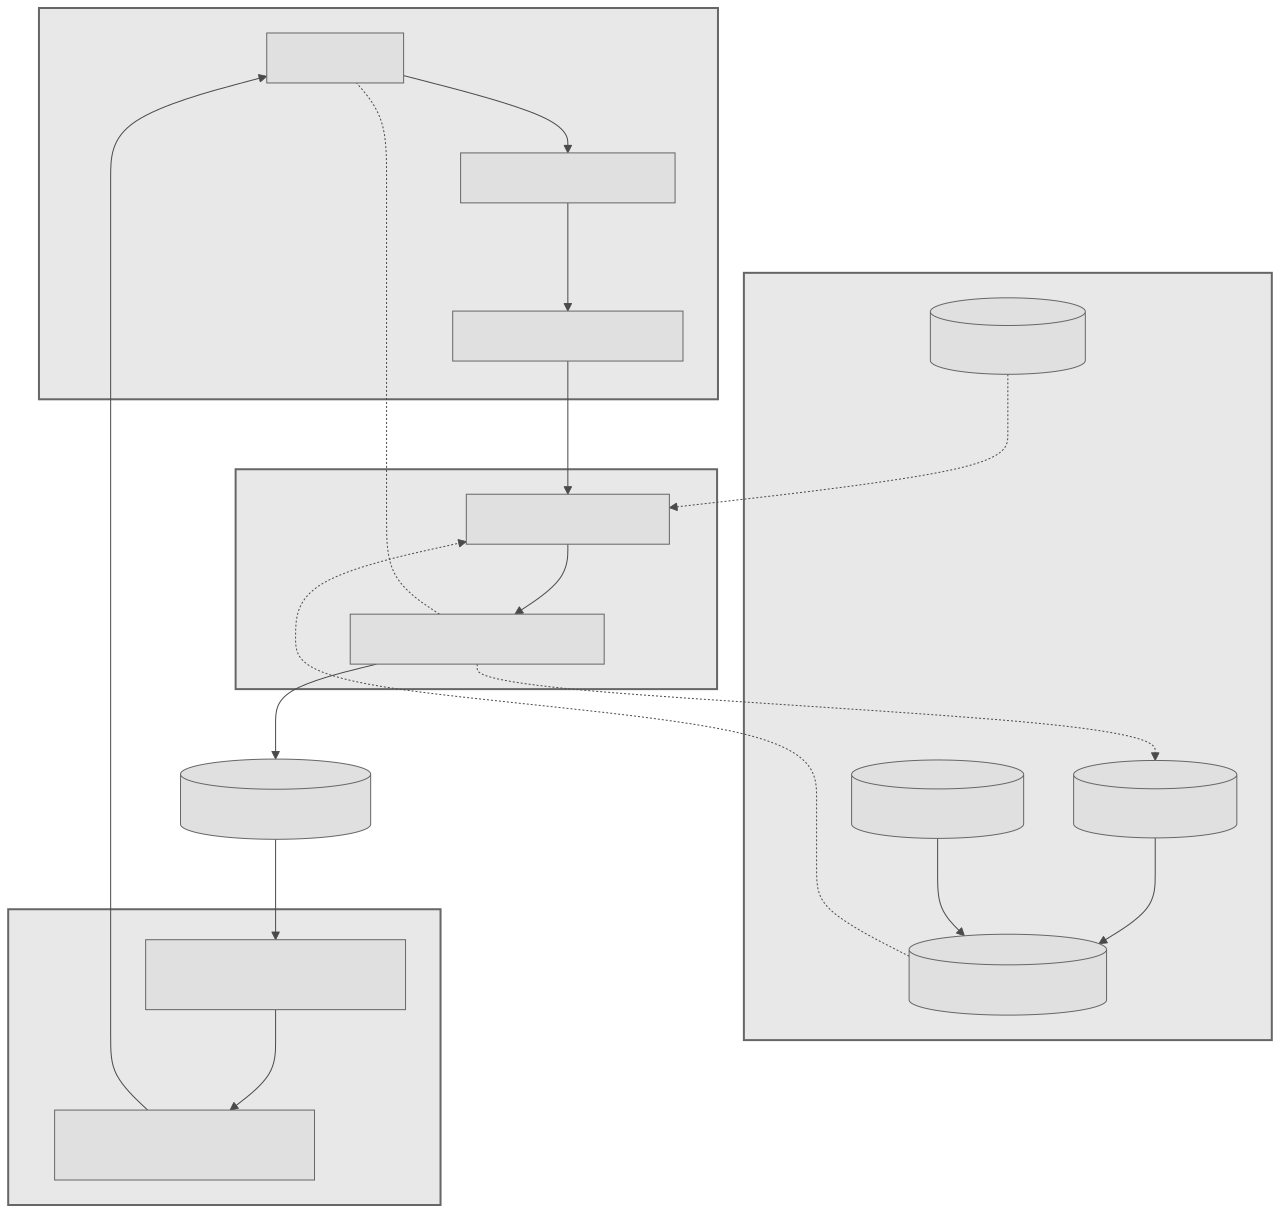
\includegraphics[width=0.95\textwidth,keepaspectratio]{figures/architecture.mmd.png}
\caption{Healthcare Analytics Architecture. Solid lines indicate the primary data flow from clinical user natural language queries through a conversational AI interface to a healthcare NLP engine for context-aware SQL generation against a healthcare data warehouse, ultimately delivering contextual insights. The critical validation step (dotted line) shows domain experts confirming or correcting generated SQL before results are trusted. Validated NL+SQL pairs flow to organizational memory (dashed line), where they persist independent of staff tenure and inform future query generation.}
\label{fig:architecture}
\end{figure}

\begin{enumerate}
\def\labelenumi{\arabic{enumi}.}
\setcounter{enumi}{2}
\tightlist
\item
  \textbf{Convergence Thesis}: The simultaneous occurrence of technical
  advances in NL2SQL, low analytics maturity, and high workforce
  turnover enables conversational AI to break the compounding cycle by
  capturing validated analytical knowledge at the point of expert
  interaction. Unlike traditional documentation that becomes stale,
  validated query pairs represent executable, tested knowledge that new
  staff can immediately use. This positions conversational AI not merely
  as a query interface but as an institutional memory preservation
  mechanism.
\end{enumerate}

\subsubsection{The Validated Query
Cycle}\label{the-validated-query-cycle}

The knowledge portal architecture preserves institutional expertise
through a six-step validated query cycle (Figure 2):

\begin{enumerate}
\def\labelenumi{\arabic{enumi}.}
\item
  \textbf{Query}: A domain expert (clinician, analyst, or administrator)
  asks a natural language question about organizational data, such as
  ``What was our 30-day readmission rate for heart failure patients last
  quarter?''
\item
  \textbf{Generation}: The conversational AI system generates candidate
  SQL code from the natural language input, leveraging healthcare
  ontologies and organizational schema knowledge to produce
  syntactically correct queries.
\item
  \textbf{Validation}: The domain expert reviews the generated SQL and
  its results, confirming correctness or providing corrections. This
  human-in-the-loop step is essential because current NL2SQL models are
  ``not yet sufficiently accurate for unsupervised use'' in clinical
  settings (\citeproc{ref-wu2024}{17}).
\item
  \textbf{Storage}: Once validated, the NL+SQL pair is stored in
  organizational memory as a durable knowledge artifact. This pair
  represents tested, executable knowledge: a verified mapping from a
  business question to the correct data retrieval logic.
\item
  \textbf{Retrieval}: When future users ask similar questions, the
  system retrieves relevant validated pairs, either returning exact
  matches or using them to inform new query generation. This reduces
  dependence on individual expertise.
\item
  \textbf{Persistence}: When the original expert leaves the
  organization, their analytical knowledge remains embedded in validated
  query pairs. New staff inherit executable knowledge rather than
  starting from scratch or relying on incomplete documentation.
\end{enumerate}

\begin{figure}[htbp]
\centering
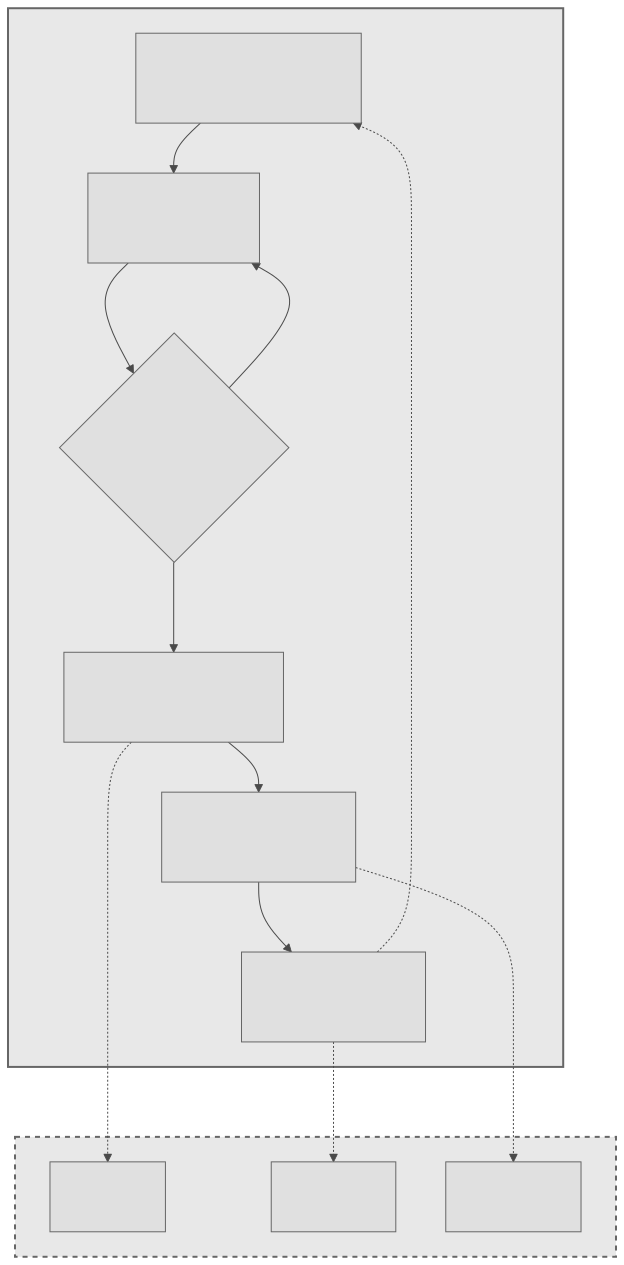
\includegraphics[width=0.5\textwidth,keepaspectratio]{figures/knowledge-cycle.mmd.png}
\caption{The Validated Query Cycle. Domain experts ask natural language questions (1), the system generates candidate SQL (2), experts validate results (3), validated pairs are stored (4), future queries retrieve validated knowledge (5), and expertise persists through staff turnover (6). This cycle breaks the compounding effect where turnover erases institutional memory.}
\label{fig:knowledge-cycle}
\end{figure}

This cycle breaks the compounding effect identified in the three-pillar
framework: turnover no longer erases analytical knowledge because
expertise is embedded in validated query pairs rather than individual
memory. Low-maturity organizations can accelerate advancement by
accumulating validated queries, and technical barriers are reduced
because new staff access proven query patterns rather than recreating
analytical logic.

\subsection{Document Structure}\label{document-structure}

Following this introduction, the paper proceeds through four main
sections. The Methodology section describes the narrative review
approach, literature search strategy, and source selection criteria. The
Literature Review synthesizes evidence across the three challenge
domains, establishing the current state of natural language processing
in healthcare, analytics maturity research, and workforce turnover
impacts. The Discussion examines implications, limitations, and future
research directions. Finally, the Conclusion summarizes the three-pillar
analytical framework as this paper's primary contribution to healthcare
informatics literature.

\section{Methodology}\label{methodology}

\subsection{Review Approach}\label{review-approach}

This paper employs a narrative review methodology to synthesize evidence
across three interconnected domains: healthcare analytics maturity,
workforce turnover, and natural language to SQL technologies. Unlike
systematic reviews that follow pre-registered protocols with exhaustive
searches, narrative reviews provide expert synthesis of relevant
literature to construct coherent arguments and identify patterns across
diverse evidence sources.

The narrative review approach was selected because:

\begin{enumerate}
\def\labelenumi{\arabic{enumi}.}
\tightlist
\item
  \textbf{Integration across domains}: The paper synthesizes evidence
  from distinct fields (clinical informatics, human resources, natural
  language processing) that require interpretive integration rather than
  statistical pooling
\item
  \textbf{Original analytical framework}: The three-pillar framework
  emerged iteratively from the literature rather than being
  pre-specified
\item
  \textbf{Heterogeneous evidence types}: The evidence base includes
  peer-reviewed research, industry reports, and benchmark datasets that
  cannot be meaningfully combined through meta-analysis
\end{enumerate}

\subsection{Literature Search}\label{literature-search}

Literature was identified through multiple channels between January 2023
and December 2025:

\textbf{Academic Databases:}

\begin{itemize}
\tightlist
\item
  Crossref: Cross-disciplinary academic literature, citation metadata
\item
  PubMed: Clinical informatics, healthcare workforce, medical
  administration
\item
  arXiv: Machine learning and NLP preprints, benchmark studies
\item
  Semantic Scholar: AI and computer science papers, citation analysis
\end{itemize}

\textbf{Industry Sources:}

\begin{itemize}
\tightlist
\item
  HIMSS: Analytics Maturity Model documentation and industry standards
\item
  Healthcare providers: NHS Trust implementation case studies
\item
  Market research: Precedence Research, Forrester analyst reports
\item
  Technology vendors: Health Catalyst, Oracle, Anthropic technical
  documentation
\item
  Professional associations: AHIMA/NORC workforce surveys
\item
  Business news: IBM, CNBC coverage of healthcare analytics ventures
\end{itemize}

\textbf{Search Concepts:}

Search terms were organized around the three-pillar framework:

\begin{itemize}
\tightlist
\item
  Analytics maturity: ``healthcare analytics maturity,'' ``HIMSS AMAM,''
  ``analytics adoption,'' ``analytics standardization failure,''
  ``low-code healthcare ROI,'' ``conversational AI platforms''
\item
  Workforce turnover: ``healthcare IT tenure,'' ``IT training time,''
  ``turnover cost salary,'' ``institutional memory loss,'' ``knowledge
  portal,'' ``knowledge capture,'' ``SECI model analytics''
\item
  Technical barriers: ``NL2SQL healthcare,'' ``text-to-SQL clinical,''
  ``MIMICSQL,'' ``EHRSQL,'' ``NL2SQL accuracy,'' ``NL2SQL
  productivity,'' ``schema discovery,'' ``PK/FK discovery,'' ``semantic
  column matching,'' ``vector embeddings schema''
\end{itemize}

\textbf{Search Results:}

Searches across all databases yielded 570 initial results after
deduplication. Crossref searches for terms including ``healthcare
analytics maturity,'' ``HIMSS AMAM,'' ``NL2SQL clinical,'' ``knowledge
portal,'' and ``low-code ROI'' (2015-current) returned 285 results, of
which 15 passed screening. PubMed searches combining workforce terms
(``healthcare IT tenure,'' ``IT training time,'' ``turnover cost
salary'') with analytics terms (``institutional memory,'' ``analytics
adoption,'' ``knowledge capture'') (2015-current) yielded 142 results
with 12 passing screening. arXiv searches in cs.CL and cs.DB categories
for ``text-to-SQL'' combined with technical terms (``MIMICSQL,''
``EHRSQL,'' ``schema discovery,'' ``PK/FK discovery,'' ``semantic
matching,'' ``vector embeddings'') (2020-current) produced 71 results
with 6 passing screening. Semantic Scholar searches for ``NL2SQL
healthcare,'' ``NL2SQL productivity,'' ``conversational AI clinical,''
and ``SECI model analytics'' (2015-current) returned 72 results with 8
passing screening. The final corpus includes 81 academic and 11 industry
sources (92 total).

Figure 3 illustrates the literature selection process, showing
progression from initial database search through screening and quality
assessment to the final corpus of 92 sources.

\begin{figure}[htbp]
\centering
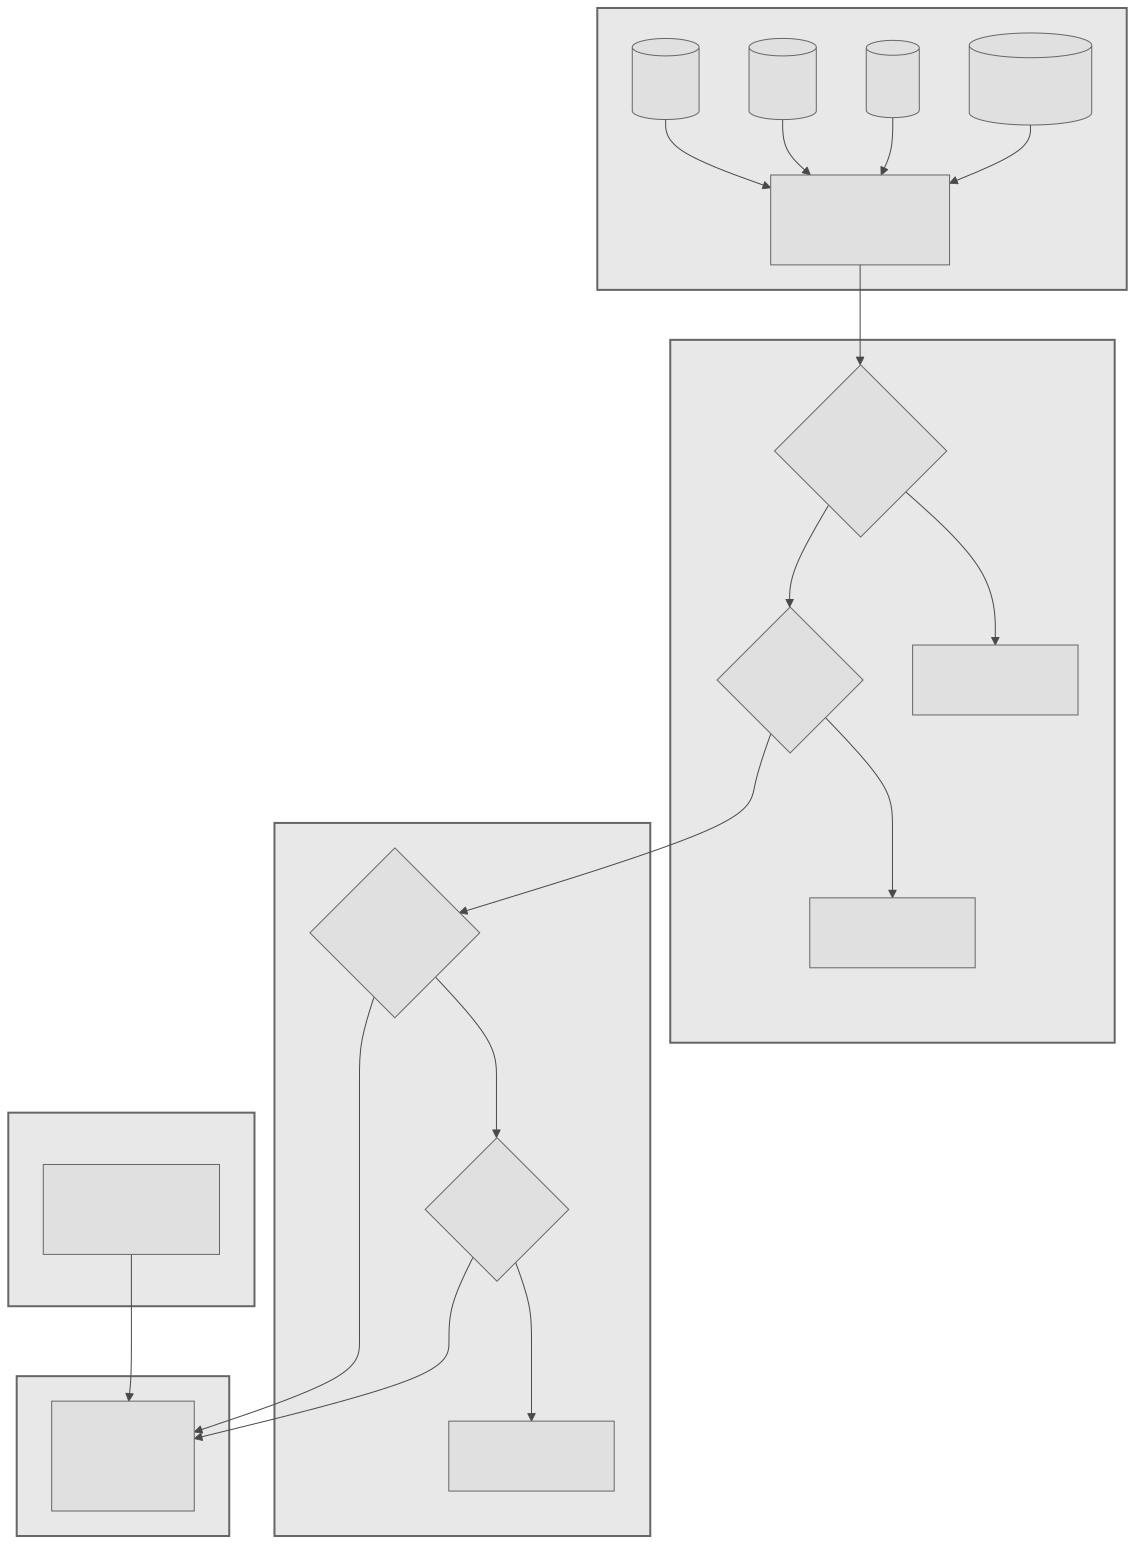
\includegraphics[width=0.9\textwidth,keepaspectratio]{figures/literature-flow.mmd.png}
\caption{Literature Selection Flow Diagram. The diagram shows the progression from initial database search (n ≈ 570) through title/abstract screening, full-text review, and quality assessment (AACODS for grey literature) to the final corpus of 92 sources (81 academic, 11 industry). Diagram source available in figures/literature-flow.mmd.}
\label{fig:literature-flow}
\end{figure}

\subsection{Source Selection}\label{source-selection}

Sources were selected based on the following criteria:

\textbf{Inclusion Criteria:}

\begin{itemize}
\tightlist
\item
  Peer-reviewed publications in healthcare informatics, medical
  informatics, computer science, or health services research
\item
  Industry reports from established healthcare IT organizations (HIMSS,
  AHIMA, AMIA)
\item
  Publications from 2015-current, with emphasis on 2020-current for
  rapidly evolving NL2SQL technologies
\item
  English language publications
\item
  Sources with verifiable DOIs, URLs, or institutional attribution
\end{itemize}

\textbf{Exclusion Criteria:}

\begin{itemize}
\tightlist
\item
  Sources without verifiable attribution or institutional backing
\item
  Vendor marketing materials without independent validation
\item
  Preprints without subsequent peer-reviewed publication (exception:
  foundational NL2SQL benchmarks where peer review is pending)
\item
  Studies with unverifiable statistics or methodological concerns
\end{itemize}

\subsection{Evidence Synthesis}\label{evidence-synthesis}

Evidence was synthesized thematically around the three-pillar framework:

\begin{enumerate}
\def\labelenumi{\arabic{enumi}.}
\tightlist
\item
  \textbf{Analytics maturity}: Evidence on HIMSS AMAM adoption,
  healthcare analytics capabilities, and organizational readiness
\item
  \textbf{Workforce turnover}: Evidence on nursing and IT staff turnover
  rates, institutional memory loss, and knowledge transfer challenges
\item
  \textbf{Technical barriers}: Evidence on NL2SQL benchmarks,
  healthcare-specific NLP challenges, and low-code implementation
  patterns
\end{enumerate}

This framework emerged iteratively from the literature rather than being
pre-specified, consistent with narrative review methodology.

\subsection{Grey Literature Quality
Assessment}\label{grey-literature-quality-assessment}

Grey literature sources were assessed using the AACODS checklist
(\citeproc{ref-tyndall2010}{18}), which evaluates Authority, Accuracy,
Coverage, Objectivity, Date, and Significance. Sources with vendor
sponsorship were retained when no independent alternative existed but
flagged in-text. Table \ref{tab:aacods} summarizes the assessment.

\begin{sidewaystable}
\centering
\caption{AACODS Assessment of Industry Sources}
\small
\begin{tabular}{|l|l|l|l|l|l|l|l|}
\hline
\textbf{Source} & \textbf{Authority} & \textbf{Accuracy} & \textbf{Coverage} & \textbf{Objectivity} & \textbf{Date} & \textbf{Significance} & \textbf{Include} \\
\hline
{[}I1{]} HIMSS AMAM & High$^\dagger$ & Verifiable & Global & High & 2024 & High & Yes \\
{[}I2{]} Snowdon/HIMSS & High$^\ddagger$ & Verifiable & N/A & High & 2024 & Medium & Yes \\
{[}I3{]} Health Catalyst & Medium$^\S$ & Unverifiable & US & Low & 2020 & Medium & Yes* \\
{[}I4{]} Berkshire NHS & High$^\P$ & Verifiable & Single site & High & 2024 & High & Yes \\
{[}I5{]} Forrester/Microsoft & Medium$^\|$ & Unverifiable & Enterprise & Low$^\diamondsuit$ & 2024 & Medium & Yes* \\
{[}I6{]} Oracle & Low$^\S$ & Unverifiable & N/A & Low & 2024 & Low & Yes* \\
{[}I7{]} Precedence Research & Medium$^\#$ & Unverifiable & Global & Medium & 2024 & Medium & Yes \\
{[}I8{]} Anthropic & Medium$^\S$ & Verifiable & N/A & Medium & 2025 & Low & Yes \\
{[}I9{]} IBM Newsroom & High$^{**}$ & Verifiable & N/A & High & 2022 & High & Yes \\
{[}I10{]} CNBC/Haven & High$^{**}$ & Verifiable & N/A & High & 2021 & High & Yes \\
{[}I11{]} AHIMA/NORC & High$^{\dagger\dagger}$ & Verifiable & US & High & 2023 & High & Yes \\
\hline
\end{tabular}
\label{tab:aacods}

\footnotesize
$^\dagger$Industry standards body.
$^\ddagger$HIMSS officer.
$^\S$Vendor.
$^\P$NHS trust.
$^\|$Analyst firm.
$^\#$Market research.
$^{**}$Journalism.
\\
$^{\dagger\dagger}$Professional association + academic.
$^\diamondsuit$Sponsor.
*Vendor sponsorship or low objectivity noted in manuscript text.
\end{sidewaystable}

\subsection{Methodological
Limitations}\label{methodological-limitations}

This narrative review has inherent limitations:

\begin{itemize}
\tightlist
\item
  \textbf{Non-exhaustive search}: Literature identification was
  selective rather than exhaustive; relevant studies may have been
  missed
\item
  \textbf{Limited formal quality assessment}: Grey literature sources
  were assessed using the AACODS checklist; however, no standardized
  quality assessment tool (e.g., GRADE, Cochrane Risk of Bias) was
  applied to peer-reviewed sources, as these tools are designed for
  clinical intervention studies rather than narrative reviews
\item
  \textbf{Single-coder bias risk}: Literature screening, data
  extraction, and thematic analysis were performed by a single author
  without independent verification. This introduces potential selection
  and interpretation bias that would be mitigated in systematic reviews
  through dual-coder protocols with inter-rater reliability assessment
\item
  \textbf{Post-hoc selection criteria}: Inclusion and exclusion criteria
  were refined during the review process rather than pre-registered
\item
  \textbf{No protocol registration}: This review was not registered in
  PROSPERO or similar registries
\item
  \textbf{Dated workforce statistics}: The primary healthcare IT
  turnover statistic (34\% annually) derives from Ang and Slaughter's
  2004 study (\citeproc{ref-ang2004}{3}). While recent surveys confirm
  workforce challenges persist (\citeproc{ref-american2023}{1}) and
  contemporary evidence suggests the situation may have worsened (55\%
  intent to leave among public health informatics specialists
  (\citeproc{ref-rajamani2025}{19})), no study has directly replicated
  the 2004 tenure measurement methodology. Future research should
  address this methodological gap
\end{itemize}

These limitations are balanced against the strengths of narrative review
methodology: ability to synthesize heterogeneous evidence types across
disciplinary boundaries, flexibility to pursue emerging themes, and
capacity to construct novel analytical frameworks that illuminate
connections between previously disconnected research domains.

\section{Framework Development and
Validation}\label{framework-development-and-validation}

This paper's primary contribution is the three-pillar analytical
framework for understanding healthcare analytics challenges: (1)
analytics maturity gaps, (2) workforce turnover and institutional memory
loss, and (3) technical barriers in natural language to SQL generation.
This section documents the framework's development process and
theoretical grounding.

\subsection{Framework Development
Process}\label{framework-development-process}

The three-pillar framework emerged through iterative analysis of the
literature corpus. Initial review identified numerous disconnected
research streams: NL2SQL technical advances, HIMSS maturity models,
healthcare workforce turnover studies, knowledge management theory, and
healthcare IT implementation case studies. These appeared as isolated
topics until thematic analysis revealed recurring patterns of
interdependence.

The framework development followed these steps:

\begin{enumerate}
\def\labelenumi{\arabic{enumi}.}
\tightlist
\item
  \textbf{Theme Extraction}: Systematic coding of 92 sources identified
  recurring themes across technical, organizational, and workforce
  dimensions
\item
  \textbf{Pattern Recognition}: Cross-domain analysis revealed that
  challenges in each dimension amplified challenges in others (e.g.,
  workforce turnover degrading analytics maturity, technical barriers
  preventing knowledge capture)
\item
  \textbf{Pillar Identification}: Three orthogonal yet interconnected
  dimensions emerged as the organizing structure:

  \begin{itemize}
  \tightlist
  \item
    \textbf{Analytics Maturity}: Organizational capability progression
    measured against HIMSS AMAM stages
  \item
    \textbf{Workforce Dynamics}: Human capital retention and tacit
    knowledge preservation
  \item
    \textbf{Technical Barriers}: NL2SQL capabilities and
    healthcare-specific implementation challenges
  \end{itemize}
\item
  \textbf{Framework Validation}: Pillar structure tested against all 92
  sources to confirm comprehensive coverage without significant gaps
\end{enumerate}

\subsection{Theoretical Grounding}\label{theoretical-grounding}

The three-pillar framework aligns with established models in healthcare
informatics and knowledge management:

\begin{table}[htbp]
\centering
\caption{Framework Alignment with Established Models}
\label{tab:framework-alignment}
\begin{tabular}{p{3cm}p{3.5cm}p{3.5cm}p{3.5cm}}
\toprule
\textbf{Three \newline Pillars} & \textbf{HIMSS AMAM Alignment} & \textbf{DIKW \newline Hierarchy} & \textbf{Knowledge Management} \\
\midrule
Analytics \newline Maturity & Stages 0-7 \newline Progression & Data \newline → Information & Organizational learning \\
Workforce \newline Dynamics & Implicit in \newline Advanced Stages & Knowledge (tacit) \newline → Wisdom & Tacit knowledge transfer \\
Technical \newline Barriers & Stage 6-7 \newline Requirements & Information \newline → Knowledge & Knowledge \newline Codification \\
\bottomrule
\end{tabular}
\end{table}

The HIMSS Analytics Maturity Assessment Model
(\citeproc{ref-himss2024}{2}) provides organizational benchmarks but
does not explicitly address workforce knowledge retention. The
Data-Information-Knowledge-Wisdom (DIKW) hierarchy explains the
progression from raw data to actionable insight, but standard
formulations do not address institutional memory loss. The three-pillar
framework synthesizes these perspectives, positioning workforce dynamics
as the critical enabler connecting data access (analytics maturity) with
organizational wisdom (knowledge preservation).

\subsection{Framework Scope and
Limitations}\label{framework-scope-and-limitations}

The framework is descriptive rather than prescriptive; it provides an
analytical lens for understanding healthcare analytics challenges but
does not mandate specific solutions. Future research should empirically
validate pillar interdependencies through longitudinal organizational
studies and develop quantitative metrics for framework dimensions.

\section{Literature Review: Natural Language Analytics in Healthcare -
Evidence for Institutional Memory
Preservation}\label{literature-review-natural-language-analytics-in-healthcare---evidence-for-institutional-memory-preservation}

This narrative review examines evidence supporting the implementation of
natural language analytics platforms in healthcare systems. Drawing from
peer-reviewed research, industry reports, and benchmark datasets
identified through the methodology described in Section 2 (Methodology),
we synthesize findings across three domains: natural language to SQL
generation, healthcare analytics maturity, and workforce dynamics.
Analysis reveals three critical findings: (1) natural language to SQL
generation has evolved significantly but faces healthcare-specific
challenges requiring specialized solutions, (2) healthcare analytics
maturity remains low with most organizations struggling at basic stages,
and (3) healthcare workforce turnover creates institutional memory loss
that traditional approaches fail to address. The evidence strongly
supports conversational AI platforms as a solution to these
interconnected challenges.

\subsection{Current State of Natural Language to SQL
Generation}\label{current-state-of-natural-language-to-sql-generation}

\subsubsection{Evolution and Technical
Advances}\label{evolution-and-technical-advances}

Recent systematic reviews document the rapid evolution of natural
language to SQL (NL2SQL) technologies. Ziletti and D'Ambrosi
(\citeproc{ref-ziletti2024}{20}) demonstrate that retrieval augmented
generation (RAG) approaches significantly improve query accuracy when
applied to electronic health records (EHRs), though they note that
``current language models are not yet sufficiently accurate for
unsupervised use'' in clinical settings; this assessment, based on 2024
models, has been challenged by late-2025 benchmarks showing GPT-5
exceeds physician baselines on standardized medical reasoning tasks
(\citeproc{ref-wang2025}{21}), (\citeproc{ref-openai2025}{22}), though
human oversight remains recommended for clinical safety. Their work on
the MIMIC-3 dataset shows that integrating medical coding steps into the
text-to-SQL process improves performance over simple prompting
approaches.

Benchmarking studies from 2024 (\citeproc{ref-medagentbench2024}{23}),
(\citeproc{ref-chen2024}{24}) examining LLM-based systems for healthcare
identify unique challenges: medical terminology, characterized by
abbreviations, synonyms, and context-dependent meanings, remains a
barrier to accurate query generation. Evaluations of GPT-4 and Claude
3.5 showed 69-73\% accuracy on clinical tasks; however, late-2025 models
demonstrate substantial improvements. GPT-5 achieves over 80\% accuracy
on neurosurgical board examinations and surpasses physician performance
on multimodal medical reasoning benchmarks by 15-29\%
(\citeproc{ref-wang2025}{21}). On healthcare-specific NL2SQL tasks,
GPT-5 achieves 64.6\% execution accuracy on the MIMICSQL dataset
(\citeproc{ref-blaskovic2025}{25}), while the HealthBench benchmark
(developed with 262 physicians across 26 specialties) shows GPT-5
hallucination rates of 0.7-1.0\%, representing a 4-6x improvement over
previous models (\citeproc{ref-openai2025}{22}).

\subsubsection{Healthcare-Specific
Challenges}\label{healthcare-specific-challenges}

The literature consistently identifies domain-specific obstacles in
healthcare NL2SQL implementation. A systematic review of NLP in EHRs
(\citeproc{ref-navarro2023}{26}) found that the lack of annotated data,
automated tools, and other challenges hinder the full utilization of NLP
for EHRs. The review, following PRISMA guidelines, categorized
healthcare NLP applications into seven areas, with information
extraction and clinical entity recognition proving most challenging due
to medical terminology complexity.

Wang et al. (\citeproc{ref-wang2020}{27}) demonstrate that healthcare
NL2SQL methods must move beyond the constraints of exact or string-based
matching to fully encompass the semantic complexities of clinical
terminology. This work emphasizes that general-purpose language models
fail to capture the nuanced relationships between medical concepts,
diagnoses codes (ICD), procedure codes (CPT), and medication
vocabularies (RxNorm).

\subsubsection{Promising Approaches and
Limitations}\label{promising-approaches-and-limitations}

Recent advances show promise in addressing these challenges. The
TREQS/MIMICSQL dataset development (\citeproc{ref-wang2020}{27}) and
EHRSQL benchmark (\citeproc{ref-lee2023}{28}) provide question-SQL pairs
specifically for healthcare, featuring questions in natural, free-form
language. Multi-modal benchmarks such as SM3-Text-to-Query
(\citeproc{ref-sivasubramaniam2024}{29}) extend evaluation beyond SQL to
support multiple query languages across diverse medical data
representations. This approach acknowledges that healthcare queries
often require multiple logical steps: population selection, temporal
relationships, aggregation statistics, and mathematical operations.

Healthcare-specific benchmarks continue to evolve alongside model
capabilities. The 2024 MedAgentBench evaluation found Claude 3.5 Sonnet
achieved 69.67\% success rate on medical agent tasks
(\citeproc{ref-medagentbench2024}{23}), (\citeproc{ref-chen2024}{24});
subsequent 2025 benchmarks show GPT-5 significantly exceeding these
results, with the SCARE benchmark (\citeproc{ref-lee2025}{30}) providing
4,200 EHR question-SQL pairs across MIMIC-III, MIMIC-IV, and eICU
databases specifically designed to evaluate post-hoc safety mechanisms
for clinical text-to-SQL deployment. Graph-empowered approaches
combining LLMs with structured knowledge representations achieve 94.2\%
execution accuracy on MIMICSQL (\citeproc{ref-chen2025}{31}),
demonstrating that domain-specific architectural innovations can
substantially outperform general-purpose models. While these advances
narrow the gap between benchmark performance and clinical readiness,
domain-specific challenges in medical terminology and complex clinical
reasoning remain active research areas.

\subsubsection{Productivity and Efficiency
Evidence}\label{productivity-and-efficiency-evidence}

Emerging research documents quantifiable productivity gains from NL2SQL
implementations. In healthcare settings, organizations implementing
natural language interfaces report a 63\% increase in self-service
analytics adoption among non-technical staff and a 37\% reduction in
time spent on data retrieval tasks (\citeproc{ref-dadi2025}{32}).
Business analysts using these interfaces spend 42\% more time on
analysis rather than query construction (\citeproc{ref-dadi2025}{32}).

Clinical-specific natural language interfaces demonstrate significant
efficiency improvements. Criteria2Query, a natural language interface
for clinical database cohort definition, achieves fully automated query
formulation in an average of 1.22 seconds per criterion, enabling
researchers to query EHR data without mastering database query languages
(\citeproc{ref-yuan2019}{33}). The system has evolved through three
generations: the original rule-based approach
(\citeproc{ref-yuan2019}{33}), a human-machine collaboration version,
and Criteria2Query 3.0, which leverages GPT-4 to generate sharable
cohort identification queries against OMOP-CDM formatted databases
(\citeproc{ref-park2024}{34}). User studies show NL2SQL systems reduce
query completion times by 10-30\% compared to traditional SQL platforms
while improving accuracy from 50\% to 75\%, with users recovering from
errors 30-40 seconds faster (\citeproc{ref-ipeirotis2025}{35}).

The most substantial productivity gains appear in multimodal interfaces.
Research on speech-driven database querying demonstrates users can
specify SQL queries with an average speedup of 2.7x (up to 6.7x)
compared to traditional input methods, with user effort reduced by a
factor of 10x to 60x compared to raw typing
(\citeproc{ref-shah2020}{36}). Healthcare-specific natural language
query systems show dramatic improvements: a clinical data analytics
language (CliniDAL) reduced complex query formulation from ``many days''
with SQL to ``a few hours'' with natural language, with expert users
describing SQL as ``very tedious and time-consuming'' for the same
analytical tasks (\citeproc{ref-safari2014}{37}). NLP-driven data entry
systems have achieved 33\% time reduction with 15\% accuracy improvement
in clinical research settings (\citeproc{ref-han2019}{38}).
Healthcare-specific NL2SQL models such as MedT5SQL achieve 80.63\% exact
match accuracy on the MIMICSQL benchmark, demonstrating that
domain-adapted language models can effectively translate natural
language to SQL for clinical databases (\citeproc{ref-marshan2024}{39}).
These metrics provide peer-reviewed evidence that complements
vendor-sponsored efficiency claims.

Code modernization principles directly inform these productivity gains.
Foundational work on natural language interfaces to databases
(\citeproc{ref-hendrix1978}{8}) established that modular, decoupled
architecture enables effective NL access to legacy systems, a design
principle applied across subsequent research (e.g.,
(\citeproc{ref-saha2023}{40})). Modern implementations demonstrate that
retrieval-augmented generation (RAG) approaches reduce specialized
training requirements by 87.4\% compared to traditional querying methods
while achieving 92.3\% accuracy in interpreting business-specific
terminology from legacy mainframe records
(\citeproc{ref-khandelwal2025}{41}). This convergence of code
modernization and natural language interface technologies arises because
both rely on the same underlying large language models
(\citeproc{ref-ogunwole2023}{9}), (\citeproc{ref-arora2025}{10}),
suggesting that organizations investing in either capability
simultaneously advance both.

\subsection{State of Healthcare Analytics
Maturity}\label{state-of-healthcare-analytics-maturity}

\subsubsection{Low Organizational
Maturity}\label{low-organizational-maturity}

The Healthcare Information Management Systems Society (HIMSS) Analytics
Maturity Assessment Model (AMAM) provides the industry standard for
measuring analytics capabilities. Recent data reveals a concerning state
of analytics maturity in healthcare organizations globally
(\citeproc{ref-himss2024}{2}). The newly revised AMAM24 model, launched
in October 2024, represents a significant evolution from the original
framework.

Snowdon (\citeproc{ref-snowdon2024b}{42}), Chief Scientific Research
Officer at HIMSS, emphasizes that ``analytics as a discipline has
changed dramatically in the last five to 10 years,'' yet healthcare
organizations struggle to keep pace (\citeproc{ref-wang2018}{4}).
Research confirms healthcare's adoption of analytics often lags behind
other sectors such as retail and banking, partly due to the complexity
of implementing new technology in clinical environments
(\citeproc{ref-wang2018}{4}), (\citeproc{ref-wang2017}{43}). The newly
revised AMAM model shifts focus from technical capabilities to outcomes,
measuring the real impact of analytics on patient care, system-wide
operations, and governance.

Quantitative evidence links organizational maturity to patient outcomes
through two related pathways. First, EMR adoption maturity provides
foundational infrastructure: cross-sectional studies using the HIMSS
Electronic Medical Record Adoption Model (EMRAM) demonstrate that
hospitals with advanced EMR adoption (levels 6-7) have 3.25 times higher
odds of achieving better Leapfrog Group Hospital Safety Grades compared
to hospitals at EMRAM level 0, with significantly reduced infection
rates and fewer adverse events (\citeproc{ref-snowdon2024}{44}).
Similarly, high-maturity hospitals have 1.8 to 2.24 times higher odds of
achieving higher patient experience ratings
(\citeproc{ref-snowdon2024a}{45}). Second, analytics capabilities build
on this digital foundation: big data analytics capabilities, combined
with complementary organizational resources and analytical personnel
skills, improve readmission rates and patient satisfaction
(\citeproc{ref-wang2019}{46}), while poor-quality data results in
diagnostic errors, ineffective treatments, and compromised patient care
(\citeproc{ref-gomes2025}{47}). Note that EMRAM measures EMR adoption
stages rather than analytics maturity directly; robust digital
infrastructure is a prerequisite for analytics, but the AMAM model
addresses the analytics-specific capability gap.

\subsubsection{Barriers to Analytics
Adoption}\label{barriers-to-analytics-adoption}

A systematic literature review of big data analytics in healthcare by
Kamble et al. (\citeproc{ref-kamble2019}{48}) identifies critical
barriers to analytics adoption. The study reveals that healthcare
enterprises struggle with technology selection, resource allocation, and
organizational readiness for data-driven decision making.

Health Catalyst's Healthcare Analytics Adoption Model
(\citeproc{ref-health2020}{49}), a vendor-produced framework,
corroborates these findings, documenting that most healthcare
organizations remain at Stages 0-3, characterized by:

\begin{itemize}
\tightlist
\item
  Fragmented data sources without integration
\item
  Limited automated reporting capabilities
\item
  Lack of standardized data governance
\item
  Minimal predictive or prescriptive analytics
\item
  Absence of real-time decision support
\end{itemize}

\subsubsection{The Analytics Skills Gap}\label{the-analytics-skills-gap}

The literature consistently identifies workforce capabilities as a
primary constraint. Healthcare organizations face mounting challenges in
extracting meaningful insights from the vast amount of unstructured
clinical text data generated daily (\citeproc{ref-navarro2023}{26}).
There is an acknowledged problem in health services where organizations
cannot make good use of available data due to a deficit in skilled
analysts across all sectors and levels (\citeproc{ref-bardsley2016}{5}).
Organizations face critical challenges in recruiting and retaining
professionals with the right analytical skills, while the need for big
data specialists with analytical capabilities continues to grow
(\citeproc{ref-pesqueira2020}{6}). Traditional approaches to analytics
require extensive technical expertise and time that healthcare
professionals typically lack, creating a fundamental barrier to
analytics adoption (\citeproc{ref-american2023}{1}).

\subsubsection{Data Quality as a Barrier to Analytics
Maturity}\label{data-quality-as-a-barrier-to-analytics-maturity}

Beyond workforce constraints, data quality represents a fundamental
barrier preventing healthcare organizations from advancing their
analytics capabilities. Research consistently demonstrates that data
quality is both a prerequisite for and a dimension of analytics
maturity; organizations cannot progress to higher maturity stages
without first addressing data quality issues
(\citeproc{ref-carvalho2019}{50}). Multiple maturity frameworks,
including the Healthcare Data Quality Maturity Model (HDQM2) and the
Data Analytics Maturity Assessment Framework (DAMAF), explicitly
incorporate data quality as a core assessment dimension
(\citeproc{ref-pintovalverde2013}{51},\citeproc{ref-gokalp2023}{52}). A
cross-industry survey found that data management and quality issues,
including lack of documentation, accuracy, and consistency, continue to
challenge analytics organizations even as they mature, with the specific
challenges shifting from integration to privacy and documentation
concerns at higher maturity levels (\citeproc{ref-lismont2017}{53}).

The prevalence of data quality issues in healthcare databases is
substantial. A study of the National Cancer Database found missing data
rates ranging from 39.7\% for prostate cancer to 71.0\% for non-small
cell lung cancer (\citeproc{ref-yang2021}{54}). Medical registry data
shows 2.0\% to 4.6\% inaccurate records and 5\% to 6\% incomplete data
(\citeproc{ref-arts2002}{55}). Duplicate patient records affect 0.16\%
to 15.47\% of records across healthcare institutions, with wide
variation in management practices (\citeproc{ref-mccoy2013}{56}).
Analysis of Medicaid claims data found that 9.74\% of data cells
contained defects, with issues frequently remaining obscure due to
separation between data users and producers
(\citeproc{ref-zhang2024}{57}).

Critically, automated data quality tools alone are insufficient for
healthcare data. Research demonstrates that clinical domain expert
involvement is necessary at every stage of the data pipeline, including
curation, cleaning, and analysis (\citeproc{ref-rahman2020}{58}).
Automated tools fail to detect context-dependent errors such as mutually
exclusive values, definitional differences between institutions, or
plausibility issues that require clinical judgment
(\citeproc{ref-sirgo2018}{59}). Even successful automation requires
embedding clinical knowledge; generic automated cleaning tools from
other domains are unsuitable for clinical data, which requires
variable-specific rules based on clinical knowledge of normal ranges,
extreme values, and clinical contexts (\citeproc{ref-shi2021}{60}).

Compounding these challenges, healthcare database schemas are frequently
undocumented or poorly documented. Commercial EMR systems use
proprietary data models that are not publicly available, requiring
``detective work'' and reverse-engineering for research data integration
(\citeproc{ref-dugas2016}{61},\citeproc{ref-bokov2017}{62}). A
systematic review found that metadata models are often too complicated
for healthcare professionals without specific IT skills, resulting in
rare usage and poorly maintained documentation
(\citeproc{ref-ulrich2022}{63}). Poor chart documentation by healthcare
providers propagates downstream to administrative data quality issues
(\citeproc{ref-lucyk2017}{64}). Most critically, documentation knowledge
is lost with staff changes: decisions based on poorly documented data
represent significant costs and risks, with explicit identification of
``loss of information with staff changes'' as a key vulnerability
(\citeproc{ref-hovenga2013}{65}).

This creates a compounding effect across the three pillars: low-maturity
organizations have worse data quality and documentation, which requires
domain expertise to address, but that expertise is lost through
workforce turnover, further degrading data quality and preventing
maturity advancement.

\subsection{Healthcare Workforce Turnover and Knowledge
Loss}\label{healthcare-workforce-turnover-and-knowledge-loss}

\subsubsection{Turnover Rates and Financial
Impact}\label{turnover-rates-and-financial-impact}

Multiple meta-analyses provide comprehensive data on healthcare
workforce turnover. Wu et al. (\citeproc{ref-wu2024}{17}) found a pooled
prevalence of nurse turnover at 18\% (95\% CI: 11-26\%), with rates
varying from 11.7\% to 46.7\% across different countries and settings.
Ren et al. (\citeproc{ref-ren2024}{66}) corroborated these findings with
a global nurse turnover rate ranging from 8\% to 36.6\%, with a pooled
rate of 16\% (95\% CI: 14-17\%).

The financial implications are substantial. Massingham
(\citeproc{ref-massingham2018}{67}) measured the impact of knowledge
loss in a longitudinal study, finding that the total financial cost to
address problems caused by knowledge loss reached three times the
organization's annual salary budget, including increased training costs,
productivity losses, and project delays. Healthcare-specific evidence
quantifies replacement costs in absolute terms: nurse turnover costs
1.2-1.3 times the registered nurse's annual salary, with the highest
cost categories being vacancy, orientation/training, and new employee
productivity loss (\citeproc{ref-jones2005}{68}); replacing a primary
care clinician costs healthcare organizations over \$500,000 due to lost
revenue and recruiting expenses (\citeproc{ref-willardgrace2019}{69});
while physician replacement can reach up to \$1 million per departure,
with national annual costs estimated at \$4.6 billion
(\citeproc{ref-melnick2021}{70}). Vendor analysis from Oracle
(\citeproc{ref-oracle2024}{71}) corroborates these findings, documenting
turnover costs at 0.5-2.0 times annual salary with knowledge-intensive
positions reaching the higher end.

Technical and analytics staff face even more severe turnover challenges.
In their 2004 study, Ang and Slaughter (\citeproc{ref-ang2004}{3}) found
that IT professionals at healthcare provider institutions (where IT
serves as a support function rather than core business) had average
tenure of just 2.9 years, implying annual turnover of 34\% (calculated
as 1/2.9 years), the highest rate among all IT organization types
studied at that time. This compared unfavorably to the 9.68-year average
for IT managerial positions overall. While this data is now two decades
old, contemporary evidence suggests the turnover challenge persists or
has worsened. A 2025 analysis of nationally representative US survey
data (n=44,732) found that 55\% of public health informatics specialists
intended to leave their positions (\citeproc{ref-rajamani2025}{19}). The
2023 AHIMA/NORC workforce survey found that 66\% of health information
professionals report persistent staffing shortages, with 83\% witnessing
increased unfilled positions over the past year
(\citeproc{ref-american2023}{1}).

The knowledge loss implications are substantial. Research documents
significant time-to-productivity requirements across healthcare IT
roles: basic EHR training requires 8 hours to 2 months for end-users,
while health information workforce development demands 18 months to 2
years for specialized roles (\citeproc{ref-ledikwe2013}{72}).
International Medical Informatics Association recommendations specify a
minimum of 1 year (60 ECTS credits) for biomedical and health
informatics specialists (\citeproc{ref-mantas2010}{73}), with
personalized EHR training programs requiring 6 months of blended
instruction to achieve meaningful competency improvements
(\citeproc{ref-musa2023}{74}). For IT developers and specialists,
research suggests up to 3 years are required to become fully fluent in
complex healthcare IT projects (\citeproc{ref-konrad2022}{75}). Combined
with the 2.9-year average tenure, healthcare IT professionals may
operate at full productivity for only approximately two years before
departing, and, in the case of IT developers, are likely to leave before
reaching full fluency. This creates a perpetual cycle where
organizations lose experienced staff before fully recouping their
training investment.

The impact on care continuity is well-documented. Clinical handover
disruption is internationally recognized as a patient safety priority
because it represents a fundamental disruption to continuity of care and
is prone to errors (\citeproc{ref-rangachari2020}{76}). Empirical
studies demonstrate that nursing unit turnover reduces workgroup
learning and is associated with increased patient falls, medication
errors, and reduced patient satisfaction (\citeproc{ref-bae2010}{77}).
International evidence links high workforce turnover to poorer
continuity of care, particularly in remote health services, with
measurable outcomes including increased hospitalizations and years of
life lost (\citeproc{ref-wakerman2019}{78}). When senior executives and
knowledge workers depart, organizations experience ``corporate memory
loss'' that undermines organizational continuity and effectiveness
(\citeproc{ref-lahaie2005}{79}).

\subsubsection{Institutional Memory
Loss}\label{institutional-memory-loss}

The concept of institutional memory in healthcare has received
increasing attention. Institutional memory encompasses the collective
knowledge, experiences, and expertise that enables organizational
effectiveness. Healthcare organizations typically lack formal mechanisms
for knowledge preservation, relying instead on person-to-person transfer
that fails during rapid turnover. Cultural and regulatory obstacles for
data sharing further limit the ability of healthcare organizations to
achieve the full potential of their data assets
(\citeproc{ref-mayo2016}{80}).

When experienced analysts, clinical informatics professionals, or
data-savvy clinicians leave, they take with them irreplaceable knowledge
about data definitions, business rules, analytical approaches, and
organizational context. Research on tacit knowledge transfer provides
strong evidence that this knowledge is inherently difficult to document
through traditional means. Empirical studies demonstrate that learning
related to tacit knowledge is often not captured in formal post-project
review reports (\citeproc{ref-goffin2011}{81}), and conventional
mechanisms such as documents, blueprints, and procedures fail because
tacit knowledge is not easily codified (\citeproc{ref-foos2006}{82}).
Research across multiple industries consistently shows that written
reports and databases fail to convey key learning from expert teams
(\citeproc{ref-goffin2010}{83}), while experts often lack the skills,
motivation, or time to document their expertise, and even when
documentation is attempted, essential aspects are lost due to lack of
shared experience between experts and novices
(\citeproc{ref-rintala2006}{84}).

\subsubsection{Inadequacy of Traditional
Approaches}\label{inadequacy-of-traditional-approaches}

The literature demonstrates that conventional knowledge management
approaches fail in healthcare contexts
(\citeproc{ref-mayo2016}{80},\citeproc{ref-shahbaz2019}{85}):

\begin{itemize}
\tightlist
\item
  Traditional knowledge transfer mechanisms show limited effectiveness
\item
  Organizations struggle to capture and maintain analytical expertise
\item
  Security concerns and employee resistance to change slow the pace of
  information system acceptance (\citeproc{ref-shahbaz2019}{85})
\item
  Person-to-person knowledge transfer fails during rapid turnover cycles
\end{itemize}

\subsection{Integration of Evidence: The Case for Conversational
AI}\label{integration-of-evidence-the-case-for-conversational-ai}

\subsubsection{Bridging Technical and Domain
Expertise}\label{bridging-technical-and-domain-expertise}

At its core, bridging technical and domain expertise serves a
fundamental patient care objective: enabling clinical professionals to
access and act on data that improves care quality. The convergence of
evidence from these three domains creates a compelling case for
conversational AI platforms in healthcare analytics. Natural language
interfaces directly address the technical barriers identified in the
literature by eliminating the need for SQL expertise while preserving
the sophisticated query capabilities required for healthcare data.

Low-code platforms and conversational AI represent complementary
approaches to reducing technical barriers in healthcare analytics.
Low-code platforms provide visual development environments that
accelerate application development and reduce coding requirements, while
conversational AI enables natural language interaction with data
systems. These approaches share core benefits: both democratize access
by enabling non-technical users to perform complex analyses previously
requiring data scientist intervention, both accelerate development
cycles by abstracting technical complexity, and both produce more
self-documenting systems where business logic is expressed in accessible
formats rather than specialized code. Evidence from low-code
implementations thus informs conversational AI adoption, as both address
the same fundamental barrier: the gap between clinical expertise and
technical capability.

\subsubsection{Knowledge Preservation
Mechanisms}\label{knowledge-preservation-mechanisms}

The literature suggests that effective knowledge preservation requires
active, embedded systems rather than passive documentation. AI-based
platforms can serve as organizational memory systems by:

\begin{itemize}
\tightlist
\item
  Capturing decision-making patterns through usage
\item
  Encoding best practices in accessible formats
\item
  Providing context-aware guidance to new users
\item
  Maintaining knowledge currency through continuous learning
\end{itemize}

These principles align with conversational AI approaches that embed
institutional knowledge within the AI model itself, making expertise
permanently accessible regardless of staff turnover.

\subsubsection{Empirical Support for Barrier-Reducing
Technologies}\label{empirical-support-for-barrier-reducing-technologies}

Academic research provides growing evidence for both conversational AI
and low-code approaches in healthcare, technologies that share the goal
of reducing technical barriers to data-driven decision making. A
foundational systematic review of AI conversational agents in healthcare
(\citeproc{ref-milneives2020}{86}) established that such systems reduce
burden on healthcare resources and save providers' time, though the
review identified a need for more rigorous quantitative validation.
Subsequent RCT-based systematic reviews provide this evidence: a
meta-analysis of conversational agent interventions reported mean task
completion rates of 83\% (range 40-100\%) across healthcare applications
(\citeproc{ref-li2023}{87}). Real-world validation at scale comes from a
study of conversational AI across nine NHS mental health services
involving 64,862 patients, demonstrating reduced clinician assessment
time, shorter patient wait times, and lower dropout rates
(\citeproc{ref-rollwage2023}{88}). On the clinical AI side, Sezgin et
al. (\citeproc{ref-sezgin2022}{89}) demonstrated that GPT-3-powered
chatbots can reduce overhead at clinics, while Jiao et al.
(\citeproc{ref-jiao2023}{90}) found AI adoption leads to cost savings
through improved service delivery and shorter hospitalization lengths.
Dai and Abramoff (\citeproc{ref-dai2023}{91}) explain that AI generates
predictions affordably, enabling earlier care that potentially prevents
costly interventions.

Low-code implementations provide parallel evidence for the benefits of
barrier reduction. Berkshire Healthcare NHS Trust
(\citeproc{ref-berkshire2024}{92}) reports over 800 ``citizen
developers'' (and over 1,600 total users) now creating solutions using
Microsoft Power Platform. The NHS program demonstrates that healthcare
professionals without IT expertise can use low-code tools to create
custom solutions and apps, streamlining operations and enabling
data-driven decisions. This evidence supports the broader principle that
reducing technical barriers, whether through visual development or
natural language interfaces, enables healthcare domain experts to
leverage data directly. A systematic literature review of 17
peer-reviewed papers identified cost and time minimization as the most
frequently discussed benefits of low-code development, with healthcare
among the primary implementation domains
(\citeproc{ref-elkamouchi2023}{93}). Controlled experiments quantify
these benefits: a comparative study of traditional versus low-code
development for a healthcare cognitive rehabilitation system found
low-code required 47.5 hours versus 888 hours for traditional
development, representing a 94.63\% reduction in effort
(\citeproc{ref-aveiro2023}{94}). Industry-sponsored research from
Forrester (\citeproc{ref-forrester2024}{95}) projects 206\% three-year
ROI from low-code implementations; peer-reviewed studies report similar
findings, with healthcare institutions achieving 177\% ROI over 36
months while reducing development time by 67\% and technical resource
requirements by 58\% (\citeproc{ref-mogili2025}{96}), and small
healthcare clinics achieving 250\% cumulative ROI over three years
(\citeproc{ref-pervaiz2025}{97}).

Healthcare-specific studies show concrete benefits across both
approaches: Pennington (\citeproc{ref-pennington2023}{98}) found AI in
revenue cycle management accelerated payment cycles from 90 days to 40
days, while Atobatele et al. (\citeproc{ref-atobatele2023}{99})
documented how low-code platforms enable non-technical staff to build
applications, leading to efficiency gains. Rapid application development
using low-code characteristics enabled an mHealth app for COVID-19
remote care that saved 2,822 hospital bed-days for 400 enrolled patients
(\citeproc{ref-tan2023}{100}). These findings collectively demonstrate
that technologies enabling non-technical users to interact with complex
systems, whether through visual interfaces or natural language, produce
measurable organizational benefits.

\subsection{Implications for Healthcare
Organizations}\label{implications-for-healthcare-organizations}

\subsubsection{Strategic Alignment with Industry
Trends}\label{strategic-alignment-with-industry-trends}

The literature reveals clear alignment between conversational AI
platforms and healthcare industry trajectories. The revised HIMSS AMAM
model (\citeproc{ref-himss2024}{2}) explicitly emphasizes AI readiness
and governance frameworks that natural language platforms inherently
support. Organizations implementing such platforms can advance multiple
maturity stages simultaneously by democratizing analytics while
maintaining governance.

\subsubsection{Return on Investment
Evidence}\label{return-on-investment-evidence}

Academic research documents multiple pathways to ROI for
barrier-reducing technologies in healthcare. Conversational AI
implementations show direct benefits: Jiao et al.
(\citeproc{ref-jiao2023}{90}) found that AI-driven efficiency gains,
including shorter hospitalization lengths, translate into financial and
operational benefits for healthcare providers; Pennington
(\citeproc{ref-pennington2023}{98}) documented that AI in revenue cycle
management accelerated payment cycles from 90 to 40 days, improving cash
flow; and Sezgin et al. (\citeproc{ref-sezgin2022}{89}) proposed chatbot
implementations that reduce clinic overhead.

Low-code platform ROI provides analogous evidence for the value of
technical barrier reduction. Industry-sponsored research from Forrester
(\citeproc{ref-forrester2024}{95}) projects 206\% three-year ROI from
Power Platform implementations. Peer-reviewed studies corroborate these
findings: a systematic review identified cost and time reduction as the
most frequently discussed benefits across 17 studies
(\citeproc{ref-elkamouchi2023}{93}), healthcare institutions report
177\% ROI over 36 months with 67\% faster development
(\citeproc{ref-mogili2025}{96}), and small healthcare clinics document
250\% cumulative three-year ROI (\citeproc{ref-pervaiz2025}{97}). While
low-code and conversational AI differ in implementation approach, both
generate returns through the same mechanism: enabling domain experts to
accomplish tasks previously requiring specialized technical staff.
Market research supports continued investment in accessible analytics:
Precedence Research (\citeproc{ref-precedence2024}{101}) projects the
healthcare analytics market to grow from \$64.49 billion in 2025 to
\$369.66 billion by 2034 (21.41\% CAGR).

\subsubsection{Risk Mitigation Through Knowledge
Preservation}\label{risk-mitigation-through-knowledge-preservation}

The literature emphasizes that institutional memory loss represents an
existential risk to healthcare analytics programs. Conversational AI
platforms mitigate this risk by transforming tacit knowledge into
encoded, accessible expertise. This approach aligns with Nonaka's SECI
model (Socialization, Externalization, Combination, Internalization),
which describes organizational knowledge creation as a continuous
dialogue between tacit and explicit knowledge
(\citeproc{ref-farnese2019}{102}). Recent research demonstrates that AI
tools can enhance all four SECI stages, particularly facilitating the
externalization process where tacit analytical knowledge becomes
explicit, queryable forms (\citeproc{ref-zhang2025}{103}). This
theoretical foundation supports embedding organizational knowledge in
systems rather than individuals, ensuring continuity despite workforce
turnover.

\subsection{Gaps in Current
Literature}\label{gaps-in-current-literature}

Despite substantial evidence supporting conversational AI in healthcare
analytics, several research gaps persist:

\begin{enumerate}
\def\labelenumi{\arabic{enumi}.}
\tightlist
\item
  \textbf{Long-term outcomes}: Most studies examine 6-24 month
  implementations; multi-year impacts remain understudied
\item
  \textbf{Scalability across specialties}: Evidence primarily focuses on
  general acute care; specialty-specific applications need investigation
\item
  \textbf{Governance frameworks}: Limited research on optimal governance
  models for democratized analytics
\item
  \textbf{Training methodologies}: Best practices for transitioning from
  traditional to conversational analytics lack empirical validation
\item
  \textbf{Integration patterns}: Architectural guidance for
  incorporating conversational AI into existing healthcare IT ecosystems
  remains sparse
\item
  \textbf{Long-term productivity tracking}: While peer-reviewed studies
  now document immediate productivity gains (63\% self-service adoption
  increase, 37\% data retrieval time reduction, 10-30\% query completion
  time improvement (\citeproc{ref-yuan2019}{33}),
  (\citeproc{ref-dadi2025}{32}), (\citeproc{ref-shah2020}{36}),
  (\citeproc{ref-ipeirotis2025}{35})), longitudinal studies tracking
  sustained productivity improvements over multiple years remain limited
\item
  \textbf{Citizen developer productivity methodology}: No validated
  healthcare-specific instrument exists for measuring citizen developer
  productivity. While Berkshire NHS reports 800+ citizen developers
  (\citeproc{ref-berkshire2024}{92}), the methodology for quantifying
  their productivity contributions lacks standardization across studies
\item
  \textbf{AMAM-specific outcome evidence}: The HIMSS Analytics Maturity
  Assessment Model (AMAM) was released in October 2024; existing outcome
  studies linking maturity stages to patient outcomes use the older
  EMRAM (EHR adoption) model
  (\citeproc{ref-snowdon2024}{44},\citeproc{ref-snowdon2024a}{45}).
  AMAM-specific outcome studies are not yet available, limiting evidence
  for analytics maturity (as distinct from EHR adoption) impact on
  outcomes
\end{enumerate}

\subsection{Why the Problem Persists}\label{why-the-problem-persists}

Despite clear evidence of healthcare's analytics challenges and
available technology, the problem remains unsolved. Analysis of market
dynamics reveals three structural barriers:

\subsubsection{Failed Standardization
Approaches}\label{failed-standardization-approaches}

Large-scale efforts to standardize healthcare data and analytics have
consistently encountered fundamental barriers. Academic research
identifies a persistent tension between achieving short-term
institutional solutions and pursuing long-term global interoperability,
with standardization complexity arising from diverse community interests
and technical issues (\citeproc{ref-richesson2007}{16}). Data
standardization faces three primary technological obstacles: metadata
uncertainties, data transfer challenges, and missing data, compounded by
legacy data collection methods that have created a ``patchwork'' of
inconsistent organizational practices (\citeproc{ref-gal2019}{104}).

These challenges manifest in clinical practice through workflow
variability. Even within the same institution, clinical workflows vary
significantly, and transitions to standardized systems often cause
profound disruptions to existing processes
(\citeproc{ref-zheng2020}{105}). At the institutional level, data
fragmentation across different organizations creates barriers to
linkage, access, and care continuity, while governance issues including
unclear responsibilities and weak collaboration compound the problem
(\citeproc{ref-bogaert2021}{106}).

High-profile industry events illustrate these documented challenges. IBM
divested its Watson Health data and analytics assets in 2022
(\citeproc{ref-ibm2022}{107}), and the Haven healthcare venture (backed
by Amazon, Berkshire Hathaway, and JPMorgan Chase) disbanded in 2021
after three years (\citeproc{ref-lavito2021}{108}). These outcomes align
with the academic literature's findings: standardized solutions face
significant barriers when applied across institutions with unique data
definitions, business rules, and clinical workflows.

These observations represent documented market events; however,
establishing causal mechanisms between organizational strategies and
interoperability outcomes requires controlled empirical research beyond
this review's scope. The patterns noted here warrant further
investigation through rigorous organizational studies.

\subsubsection{Deployment Constraint
Mismatch}\label{deployment-constraint-mismatch}

Healthcare organizations increasingly require solutions functional in
secure, air-gapped environments due to regulatory requirements and data
governance policies. General-purpose cloud AI services cannot meet these
deployment constraints while simultaneously lacking the
institution-specific context necessary for accurate analytics. The
fundamental requirement that institutional knowledge must be captured,
preserved, and accessed within each organization's specific environment
cannot be addressed by standardized cloud offerings.

These dynamics explain why, despite technological capability, the
healthcare analytics maturity gap persists. Solutions must be designed
for institution-specific deployment rather than cross-organizational
standardization.

\section{Discussion}\label{discussion}

\subsection{Strengths of the Evidence
Base}\label{strengths-of-the-evidence-base}

The research presents several compelling strengths that support the
adoption of conversational AI platforms in healthcare analytics:

\subsubsection{Validated Benchmarking
Data}\label{validated-benchmarking-data}

The evidence base includes peer-reviewed benchmarking studies from top
venues (NEJM AI, NeurIPS, NAACL) that provide empirical validation of
LLM capabilities in healthcare contexts. Studies like MedAgentBench
(\citeproc{ref-medagentbench2024}{23}) and comprehensive medical LLM
evaluations (\citeproc{ref-chen2024}{24}) offer reproducible,
quantitative performance metrics.

\subsubsection{Real-World Implementation
Evidence}\label{real-world-implementation-evidence}

The Berkshire Healthcare NHS Trust case
(\citeproc{ref-berkshire2024}{92}) demonstrates successful low-code
adoption in healthcare, with over 800 citizen developers creating
solutions. This provides concrete evidence that non-technical healthcare
professionals can effectively use these platforms.

\subsubsection{Addresses Multiple Challenges
Simultaneously}\label{addresses-multiple-challenges-simultaneously}

Unlike point solutions that address individual problems, conversational
AI platforms simultaneously tackle technical barriers, analytics
maturity constraints, and institutional memory loss. This integrated
approach enables healthcare organizations to advance multiple capability
areas with a single strategic investment.

\subsubsection{Strong Economic
Justification}\label{strong-economic-justification}

The financial evidence is compelling, with Forrester Research
(\citeproc{ref-forrester2024}{95}) documenting 206\% three-year ROI from
low-code implementations. Market growth projections
(\citeproc{ref-precedence2024}{101}) showing the healthcare analytics
market expanding from \$64.49B to \$369.66B by 2034 indicate sustained
investment demand.

\subsubsection{Honest Assessment of
Limitations}\label{honest-assessment-of-limitations}

The evidence base includes important caveats. Ziletti and D'Ambrosi
(\citeproc{ref-ziletti2024}{20}) note that ``current language models are
not yet sufficiently accurate for unsupervised use,'' and benchmarking
studies (\citeproc{ref-ang2004}{3},\citeproc{ref-chen2024}{24}) show
significant gaps between benchmark performance and clinical readiness.
This honest assessment enables appropriate implementation strategies.

\subsection{Limitations and
Constraints}\label{limitations-and-constraints}

Despite strong evidence supporting conversational AI adoption, several
limitations must be acknowledged:

\subsubsection{Implementation
Complexity}\label{implementation-complexity}

Healthcare environments present unique complexity challenges including
regulatory requirements, legacy system integration, and change
management across diverse user populations. Implementation timelines
reflect this complexity, though low-code approaches compare favorably to
traditional analytics infrastructure projects. Healthcare and
pharmaceutical organizations face particularly acute legacy
modernization challenges, paralleling patterns documented in broader
enterprise software contexts (\citeproc{ref-anthropic2025}{7}).

\subsubsection{Context-Specific Customization
Requirements}\label{context-specific-customization-requirements}

Healthcare organizations vary significantly in data structures, clinical
workflows, and analytical needs. Evidence suggests that successful
implementations require substantial customization to organizational
contexts, potentially limiting the applicability of standardized
approaches.

\subsubsection{Long-Term Outcome
Uncertainties}\label{long-term-outcome-uncertainties}

Most studies examine 6-24 month implementations. Questions remain about
long-term sustainability, user engagement over extended periods, and the
evolution of organizational capabilities beyond initial deployment
periods. The research gap analysis in the Literature Review identifies
this as a priority area for future investigation.

\subsubsection{Governance and Quality Assurance
Challenges}\label{governance-and-quality-assurance-challenges}

Democratizing analytics access creates new challenges in maintaining
data quality, analytical rigor, and clinical safety standards. While the
evidence shows reduced error rates with conversational AI, healthcare
organizations must develop new governance frameworks for managing
distributed analytical capabilities.

\subsubsection{Specialty-Specific Application
Gaps}\label{specialty-specific-application-gaps}

Evidence primarily focuses on general acute care settings. Applications
in specialized domains (oncology, cardiology, mental health) require
domain-specific validation and customization that may not generalize
from the existing evidence base.

\subsubsection{Methodological
Considerations}\label{methodological-considerations}

As a narrative review, this paper has methodological limitations
distinct from systematic reviews. The non-exhaustive literature search,
single-author synthesis, and post-hoc selection criteria may have
introduced selection or interpretation bias. No formal quality
assessment tool was applied to included studies. These limitations,
documented in detail in the Methodology section, should be considered
when interpreting findings. The transparency provided through explicit
documentation of search strategies, selection criteria, and synthesis
approach enables readers to assess potential biases and evaluate the
robustness of conclusions.

\subsection{Future Research
Directions}\label{future-research-directions}

The evidence review identifies several priority areas for future
investigation:

\subsubsection{Short-Term Research Priorities (\textless1
year)}\label{short-term-research-priorities-1-year}

\begin{enumerate}
\def\labelenumi{\arabic{enumi}.}
\tightlist
\item
  \textbf{Reference Implementation Validation}: Empirical validation of
  NL2SQL approaches using synthetic healthcare data (e.g., Synthea) in
  reproducible cloud environments, enabling benchmarking against
  established datasets (EHRSQL, MIMICSQL) without privacy constraints
\item
  \textbf{Schema Discovery for Healthcare Databases}: Research on
  automated primary/foreign key discovery algorithms applied to
  healthcare schemas, addressing the complexity of clinical data models
\item
  \textbf{Governance Framework Development}: Research on optimal
  governance models for democratized analytics
\end{enumerate}

\subsubsection{Medium-Term Research Priorities (1-2
years)}\label{medium-term-research-priorities-1-2-years}

\begin{enumerate}
\def\labelenumi{\arabic{enumi}.}
\tightlist
\item
  \textbf{Healthcare Terminology Integration}: Development of
  programmatic approaches for mapping natural language queries to
  standardized vocabularies (SNOMED CT, LOINC, RxNorm) within NL2SQL
  pipelines
\item
  \textbf{FHIR/OMOP Interoperability}: Research on reducing ETL burden
  for OMOP Common Data Model and FHIR transformations, enabling NL2SQL
  systems to operate across heterogeneous healthcare data standards
\item
  \textbf{Longitudinal Outcome Studies}: Multi-year implementations to
  assess sustained benefits and organizational evolution
\item
  \textbf{Comparative Effectiveness Research}: Head-to-head comparisons
  of different conversational AI approaches on healthcare-specific
  benchmarks
\end{enumerate}

\subsubsection{Long-Term Research Priorities (\textgreater2
years)}\label{long-term-research-priorities-2-years}

\begin{enumerate}
\def\labelenumi{\arabic{enumi}.}
\tightlist
\item
  \textbf{Organizational Transformation Studies}: Research on how
  conversational AI platforms reshape healthcare organizational
  capabilities
\item
  \textbf{Clinical Outcome Impact Assessment}: Studies linking improved
  analytics access to patient care outcomes
\item
  \textbf{Cross-Institution Knowledge Portals}: Investigation of
  federated approaches enabling knowledge sharing across healthcare
  organizations while maintaining privacy and security requirements
\end{enumerate}

\subsection{The Validated Query Cycle as Knowledge
Preservation}\label{the-validated-query-cycle-as-knowledge-preservation}

The validated query cycle introduced in this paper differs fundamentally
from traditional knowledge management approaches in healthcare.
Traditional approaches rely on documentation: analysts write procedures,
create data dictionaries, and maintain query libraries. However,
documentation suffers from three critical weaknesses: it becomes stale
as systems evolve, it captures procedural knowledge but not contextual
judgment, and it requires active maintenance that often lapses after
staff transitions.

Validated query pairs address each weakness. First, validated pairs are
executable: they can be tested against current data to verify continued
correctness, unlike static documentation. Second, validated pairs
capture the complete mapping from business question to data retrieval
logic, embedding the contextual judgment that documentation typically
omits (why this join, why this filter, why this aggregation). Third,
validation happens at the point of use rather than as a separate
maintenance task: every confirmed query becomes a knowledge artifact
without additional documentation effort.

This mechanism also differs from traditional query logging or usage
analytics. Query logs capture what was asked, but not whether the answer
was correct. Validated query pairs capture expert confirmation that the
SQL correctly answers the business question. This distinction is
critical for institutional memory: organizations need to know not just
what queries were run, but which queries produced trusted, verified
answers.

Governance requirements for the validated query cycle include: defining
who can validate queries (domain expertise requirements), establishing
validation workflows (review processes for high-stakes queries),
managing query versioning (as schemas evolve), and implementing
retrieval policies (when to return exact matches versus inform new
generation). Organizations implementing conversational AI platforms
should design these governance structures before deployment rather than
retrofitting them after knowledge accumulation begins.

\subsection{Implications for Healthcare
Organizations}\label{implications-for-healthcare-organizations-1}

The evidence has implications for healthcare leaders considering
analytics strategy:

\subsubsection{Organizational Assessment Using the Three-Pillar
Framework}\label{organizational-assessment-using-the-three-pillar-framework}

The three-pillar framework provides a structured approach for
organizational self-assessment:

\begin{enumerate}
\def\labelenumi{\arabic{enumi}.}
\tightlist
\item
  \textbf{Analytics Maturity Assessment}: Where does the organization
  currently stand on the HIMSS AMAM scale? What capabilities are needed
  to advance?
\item
  \textbf{Workforce Knowledge Audit}: What tacit knowledge resides with
  individual staff members? How vulnerable is the organization to
  knowledge loss through turnover?
\item
  \textbf{Technical Barrier Inventory}: What technical skills are
  currently required for data access? Which clinical questions go
  unanswered due to technical barriers?
\end{enumerate}

\subsubsection{Three-Pillar Assessment
Rubric}\label{three-pillar-assessment-rubric}

The three-pillar framework enables organizational self-assessment to
determine readiness for and potential benefit from NL2SQL and
conversational AI interventions. Table 3 provides an evidence-based
rubric where each indicator anchors to reviewed literature.
Organizations scoring predominantly ``Higher Risk'' across pillars face
compounding challenges that NL2SQL platforms are specifically designed
to address: democratizing data access (Technical Barriers), preserving
institutional knowledge (Workforce Dynamics), and accelerating maturity
advancement (Analytics Maturity).

\textbf{Table 3: Three-Pillar Organizational Assessment Rubric}

\textbf{Analytics Maturity Indicators:}

\begin{longtable}[]{@{}
  >{\raggedright\arraybackslash}p{(\columnwidth - 8\tabcolsep) * \real{0.1803}}
  >{\raggedright\arraybackslash}p{(\columnwidth - 8\tabcolsep) * \real{0.1967}}
  >{\raggedright\arraybackslash}p{(\columnwidth - 8\tabcolsep) * \real{0.2459}}
  >{\raggedright\arraybackslash}p{(\columnwidth - 8\tabcolsep) * \real{0.2131}}
  >{\raggedright\arraybackslash}p{(\columnwidth - 8\tabcolsep) * \real{0.1639}}@{}}
\toprule\noalign{}
\begin{minipage}[b]{\linewidth}\raggedright
Indicator
\end{minipage} & \begin{minipage}[b]{\linewidth}\raggedright
Lower Risk
\end{minipage} & \begin{minipage}[b]{\linewidth}\raggedright
Moderate Risk
\end{minipage} & \begin{minipage}[b]{\linewidth}\raggedright
Higher Risk
\end{minipage} & \begin{minipage}[b]{\linewidth}\raggedright
Evidence
\end{minipage} \\
\midrule\noalign{}
\endhead
\bottomrule\noalign{}
\endlastfoot
HIMSS AMAM Stage & Stages 5-7: Predictive analytics, AI integration &
Stages 3-4: Integrated warehouse, standardized definitions & Stages 0-2:
Fragmented data, limited reporting &
(\citeproc{ref-himss2024}{2},\citeproc{ref-health2020}{49}) \\
Self-service analytics & Widespread; clinical staff access data directly
& Partial; BI tools available but underutilized & None; all analytics
require IT intervention &
(\citeproc{ref-wang2018}{4},\citeproc{ref-berkshire2024}{92}) \\
AI/NL interface availability & Natural language query capability
deployed & Pilot programs or evaluation underway & No NL2SQL or
conversational analytics &
(\citeproc{ref-ziletti2024}{20},\citeproc{ref-wang2020}{27}) \\
\end{longtable}

\textbf{Workforce Dynamics Indicators:}

\begin{longtable}[]{@{}
  >{\raggedright\arraybackslash}p{(\columnwidth - 8\tabcolsep) * \real{0.1803}}
  >{\raggedright\arraybackslash}p{(\columnwidth - 8\tabcolsep) * \real{0.1967}}
  >{\raggedright\arraybackslash}p{(\columnwidth - 8\tabcolsep) * \real{0.2459}}
  >{\raggedright\arraybackslash}p{(\columnwidth - 8\tabcolsep) * \real{0.2131}}
  >{\raggedright\arraybackslash}p{(\columnwidth - 8\tabcolsep) * \real{0.1639}}@{}}
\toprule\noalign{}
\begin{minipage}[b]{\linewidth}\raggedright
Indicator
\end{minipage} & \begin{minipage}[b]{\linewidth}\raggedright
Lower Risk
\end{minipage} & \begin{minipage}[b]{\linewidth}\raggedright
Moderate Risk
\end{minipage} & \begin{minipage}[b]{\linewidth}\raggedright
Higher Risk
\end{minipage} & \begin{minipage}[b]{\linewidth}\raggedright
Evidence
\end{minipage} \\
\midrule\noalign{}
\endhead
\bottomrule\noalign{}
\endlastfoot
Annual IT turnover rate & \textless15\% & 15-30\% & \textgreater30\%
(exceeds 2004 healthcare IT baseline) & (\citeproc{ref-ang2004}{3}) \\
Knowledge concentration & Distributed expertise; documented processes &
Partial documentation; some cross-training & Critical expertise held by
≤3 individuals &
(\citeproc{ref-benbya2004}{15},\citeproc{ref-richesson2007}{16}) \\
Time-to-productivity & \textless6 months with structured onboarding &
6-18 months & \textgreater18 months (specialized health informatics
roles) &
(\citeproc{ref-ledikwe2013}{72}--\citeproc{ref-musa2023}{74}) \\
Tacit knowledge capture & Expertise embedded in systems/AI & Partial
documentation exists & Person-dependent; undocumented tribal knowledge &
(\citeproc{ref-benbya2004}{15}) \\
\end{longtable}

\textbf{Technical Barriers Indicators:}

\begin{longtable}[]{@{}
  >{\raggedright\arraybackslash}p{(\columnwidth - 8\tabcolsep) * \real{0.1803}}
  >{\raggedright\arraybackslash}p{(\columnwidth - 8\tabcolsep) * \real{0.1967}}
  >{\raggedright\arraybackslash}p{(\columnwidth - 8\tabcolsep) * \real{0.2459}}
  >{\raggedright\arraybackslash}p{(\columnwidth - 8\tabcolsep) * \real{0.2131}}
  >{\raggedright\arraybackslash}p{(\columnwidth - 8\tabcolsep) * \real{0.1639}}@{}}
\toprule\noalign{}
\begin{minipage}[b]{\linewidth}\raggedright
Indicator
\end{minipage} & \begin{minipage}[b]{\linewidth}\raggedright
Lower Risk
\end{minipage} & \begin{minipage}[b]{\linewidth}\raggedright
Moderate Risk
\end{minipage} & \begin{minipage}[b]{\linewidth}\raggedright
Higher Risk
\end{minipage} & \begin{minipage}[b]{\linewidth}\raggedright
Evidence
\end{minipage} \\
\midrule\noalign{}
\endhead
\bottomrule\noalign{}
\endlastfoot
Data access requirements & Natural language or visual query interfaces &
IT queue for complex queries; basic self-service & SQL/technical
expertise required for all queries &
(\citeproc{ref-wang2018}{4}--\citeproc{ref-pesqueira2020}{6}) \\
Interoperability status & Unified data platform; real-time integration &
Partial integration; some automated feeds & Fragmented systems; manual
reconciliation required &
(\citeproc{ref-gal2019}{104},\citeproc{ref-bogaert2021}{106}) \\
Skills gap severity & Sufficient analysts across departments &
Acknowledged deficit with mitigation plans & Critical shortage
preventing data utilization &
(\citeproc{ref-bardsley2016}{5},\citeproc{ref-pesqueira2020}{6}) \\
\end{longtable}

\textbf{Convergence Assessment and NL2SQL Indication:}

\begin{longtable}[]{@{}
  >{\raggedright\arraybackslash}p{(\columnwidth - 4\tabcolsep) * \real{0.3288}}
  >{\raggedright\arraybackslash}p{(\columnwidth - 4\tabcolsep) * \real{0.1644}}
  >{\raggedright\arraybackslash}p{(\columnwidth - 4\tabcolsep) * \real{0.5068}}@{}}
\toprule\noalign{}
\begin{minipage}[b]{\linewidth}\raggedright
Organizational Profile
\end{minipage} & \begin{minipage}[b]{\linewidth}\raggedright
Assessment
\end{minipage} & \begin{minipage}[b]{\linewidth}\raggedright
NL2SQL/Conversational AI Relevance
\end{minipage} \\
\midrule\noalign{}
\endhead
\bottomrule\noalign{}
\endlastfoot
All pillars Lower Risk & Continuous improvement stance & Opportunistic;
enhancement rather than necessity \\
1 pillar Higher Risk & Targeted intervention needed & Address specific
pillar; monitor for spillover \\
2 pillars Higher Risk & Compounding effects likely & Strong indication
for comprehensive assessment \\
All 3 pillars Higher Risk & Self-reinforcing degradation cycle & Urgent
evaluation warranted; NL2SQL addresses all three dimensions
simultaneously \\
\end{longtable}

NL2SQL platforms specifically target the convergence condition: they
reduce Technical Barriers by eliminating SQL requirements, mitigate
Workforce Dynamics risks by encoding expertise in queryable systems, and
accelerate Analytics Maturity by enabling citizen developer
participation (\citeproc{ref-berkshire2024}{92}). Organizations at
Higher Risk across multiple pillars represent the primary use case for
conversational AI adoption.

\subsubsection{Implementation
Considerations}\label{implementation-considerations}

Evidence from healthcare implementations suggests several factors
influence success:

\begin{itemize}
\tightlist
\item
  \textbf{Governance Framework Development}: New policies and procedures
  for democratized analytics
\item
  \textbf{Change Management}: Training and support programs to ensure
  user adoption
\item
  \textbf{Phased Deployment}: Gradual rollout beginning with
  analytics-savvy early adopters
\item
  \textbf{Human Oversight}: Current NL2SQL limitations require
  maintaining human review of AI-generated outputs
  (\citeproc{ref-ziletti2024}{20})
\end{itemize}

\section{Conclusion}\label{conclusion}

This narrative review synthesized evidence across three interconnected
domains: natural language to SQL generation, healthcare analytics
maturity, and workforce-driven institutional memory loss. The findings
illuminate a tension central to healthcare's approach to emerging
technologies, captured in the ancient principle \emph{primum non
nocere}: ``First, do no harm.''

\subsection{The Dual Dimensions of
Harm}\label{the-dual-dimensions-of-harm}

Healthcare's traditional interpretation of \emph{primum non nocere}
counsels caution: new technologies should be thoroughly validated before
clinical deployment, and governance frameworks should default to
rejection until safety is established. This principle has served
healthcare well, protecting patients from unproven interventions and
maintaining professional standards.

However, the evidence reviewed in this paper suggests that \emph{primum
non nocere} must be applied bidirectionally. The three-pillar analysis
reveals substantial harms from \textbf{inaction}:

\begin{itemize}
\tightlist
\item
  \textbf{Analytics maturity gaps} leave clinical decisions unsupported
  by available data, directly impacting patient care quality and safety
\item
  \textbf{Workforce turnover} (34\% annually for healthcare IT staff as
  of 2004 (\citeproc{ref-ang2004}{3})) causes institutional memory loss
  that disrupts care continuity and erodes the knowledge base essential
  for quality improvement
\item
  \textbf{Technical barriers} disconnect clinical experts from data
  insights, preventing evidence-based practice improvements that could
  benefit patients
\end{itemize}

These findings do not argue that healthcare organizations should abandon
caution. Rather, they suggest that a complete application of
\emph{primum non nocere} requires evaluating \textbf{both} the risks of
premature technology adoption \textbf{and} the ongoing harms of
maintaining current approaches. The three-pillar framework presented in
this review provides a structured approach for this dual evaluation.

\subsection{Summary of Contributions}\label{summary-of-contributions}

This narrative review contributes to healthcare informatics scholarship
through:

\begin{enumerate}
\def\labelenumi{\arabic{enumi}.}
\item
  \textbf{Novel Analytical Framework}: The three-pillar framework
  synthesizes previously disconnected evidence from healthcare analytics
  maturity, workforce management, and natural language processing
  research, revealing how these challenges interconnect and compound
  each other: low maturity accelerates turnover, turnover degrades
  maturity, and technical barriers prevent recovery from either.
\item
  \textbf{Knowledge Portal Application}: By applying established
  knowledge portal theory
  (\citeproc{ref-benbya2004}{15},\citeproc{ref-richesson2007}{16}) to
  healthcare conversational AI, we provide a conceptual foundation for
  institutional memory preservation systems that embed organizational
  expertise within AI platforms rather than individual staff.
\item
  \textbf{Convergence Thesis}: The simultaneous occurrence of technical
  advances in NL2SQL, organizational analytics challenges, and workforce
  dynamics creates conditions requiring active organizational
  assessment. This convergence transforms the technology adoption
  question from a matter of preference to one with institutional
  knowledge preservation implications, warranting structured evaluation
  using frameworks such as the three-pillar model.
\end{enumerate}

\subsection{Key Findings}\label{key-findings}

This review of academic and industry sources establishes several
critical findings:

\begin{enumerate}
\def\labelenumi{\arabic{enumi}.}
\item
  \textbf{Technical Progress with Limitations}: Natural language to SQL
  technologies have advanced significantly, with healthcare-specific
  benchmarks (\citeproc{ref-wang2020}{27},\citeproc{ref-lee2023}{28})
  demonstrating substantial progress in clinical NL2SQL tasks. However,
  current models are ``not yet sufficiently accurate for unsupervised
  use'' in clinical settings (\citeproc{ref-ziletti2024}{20}), requiring
  human oversight.
\item
  \textbf{Organizational Need}: Healthcare analytics maturity remains an
  ongoing challenge, with the revised HIMSS AMAM model
  (\citeproc{ref-himss2024}{2}) emphasizing the need for AI readiness
  and governance frameworks. Most organizations struggle to advance
  beyond basic reporting levels.
\item
  \textbf{Workforce Impact}: Healthcare IT staff turnover was measured
  at 34\% in 2004 (\citeproc{ref-ang2004}{3}), the highest among IT
  sectors at that time, and workforce challenges persist today
  (\citeproc{ref-american2023}{1}). Knowledge loss costs can reach three
  times annual salary budgets (\citeproc{ref-massingham2018}{67}),
  creating need for knowledge preservation approaches.
\item
  \textbf{Implementation Evidence}: Real-world implementations like
  Berkshire Healthcare NHS Trust (\citeproc{ref-berkshire2024}{92})
  demonstrate that low-code platforms can enable 800+ citizen developers
  in healthcare settings, with academic research documenting significant
  efficiency improvements and cost reductions
  (\citeproc{ref-sezgin2022}{89},\citeproc{ref-jiao2023}{90}).
\end{enumerate}

\subsection{Implications for Organizational
Assessment}\label{implications-for-organizational-assessment}

The evidence synthesis suggests healthcare organizations face decisions
that cannot be reduced to simple adoption/rejection binaries. Applying
\emph{primum non nocere} comprehensively requires organizational leaders
to:

\begin{enumerate}
\def\labelenumi{\arabic{enumi}.}
\item
  \textbf{Assess current harm exposure}: Quantify institutional memory
  loss from turnover, measure time-to-insight for clinical questions,
  and evaluate analytics capability gaps against organizational needs
\item
  \textbf{Evaluate intervention risks}: Consider NL2SQL accuracy
  limitations (``not yet sufficiently accurate for unsupervised use''
  (\citeproc{ref-ziletti2024}{20})), governance requirements, and
  implementation complexity
\item
  \textbf{Apply the three-pillar framework}: Use the analytics maturity,
  workforce turnover, and technical barrier dimensions to structure
  organizational assessment and prioritization
\end{enumerate}

Throughout this assessment, quality patient care must remain the primary
metric. Operational efficiency, cost savings, and technical capabilities
are valuable only insofar as they advance healthcare's fundamental
mission.

This framework acknowledges that optimal decisions will vary by
organizational context. Healthcare systems with stable analytics teams
and mature data infrastructure face different risk profiles than those
experiencing rapid turnover and limited analytics capabilities. The
evidence does not prescribe universal solutions but provides structured
approaches for context-specific evaluation.

\subsection{Closing Reflection}\label{closing-reflection}

\emph{Primum non nocere} ultimately requires healthcare organizations to
make evidence-based judgments about both action and inaction. This
review contributes a three-pillar analytical framework to support those
judgments, synthesizing evidence on analytics maturity, workforce
dynamics, and technical capabilities.

The evidence does not prescribe universal adoption of any technology.
Rather, it establishes the scope and interconnection of challenges that
organizations must address through whatever means align with their
specific contexts, capabilities, and risk tolerances. The ongoing harms
documented in this review (institutional memory loss, analytics
capability gaps, and technical barriers to data access) merit the same
careful consideration as the risks of new technology adoption.

Healthcare's commitment to avoiding harm is best served by
evidence-based evaluation that considers all dimensions of potential
benefit and risk. The three-pillar framework offers one structured
approach for conducting such evaluations.

\section{Acknowledgments}\label{acknowledgments}

The author (S.T.H.) takes full responsibility for the final content,
conducted the research, and verified all claims and citations. Claude
Code (Claude Opus 4.5, Anthropic) assisted with manuscript editing and
refinement.

\section{Author Contributions}\label{author-contributions}

S.T.H. conceived the research, conducted the literature review, and
wrote the manuscript.

\section{Conflicts of Interest}\label{conflicts-of-interest}

The author declares the following competing interests: Samuel T Harrold
is a contract product advisor at Yuimedi, Inc., which develops
healthcare analytics software including conversational AI platforms
relevant to this review's subject matter. The author is also employed as
a Data Scientist at Indiana University Health. This paper presents an
analytical framework derived from published literature and does not
evaluate or recommend specific commercial products, including those of
the author's affiliated organizations. The views expressed are the
author's own and do not represent the official positions of Indiana
University Health or Yuimedi, Inc.

\section{Data Availability}\label{data-availability}

This is a narrative review synthesizing existing literature. No primary
datasets were generated or analyzed. All data cited are from publicly
available peer-reviewed publications and industry reports, referenced in
the bibliography. The literature search methodology and source selection
criteria are documented in the Methodology section.

\section{Code Availability}\label{code-availability}

Not applicable. No custom code was developed for this research.

\section{Funding}\label{funding}

Yuimedi provided funding for the author's time writing and researching
this manuscript.

\section{Abbreviations}\label{abbreviations}

AACODS: Authority, Accuracy, Coverage, Objectivity, Date, Significance
ACO: Accountable Care Organization AI: Artificial Intelligence AMAM:
Analytics Maturity Assessment Model CPT: Current Procedural Terminology
DAMAF: Data Analytics Maturity Assessment Framework DIKW:
Data-Information-Knowledge-Wisdom EHR: Electronic Health Record EMRAM:
Electronic Medical Record Adoption Model HDQM2: Healthcare Data Quality
Maturity Model HIMSS: Healthcare Information Management Systems Society
ICD: International Classification of Diseases IT: Information Technology
LLM: Large Language Model NL2SQL: Natural Language to SQL RAG:
Retrieval-Augmented Generation SQL: Structured Query Language

\section{Appendices}\label{appendices}

\subsection{Appendix A: Healthcare Analytics
Glossary}\label{appendix-a-healthcare-analytics-glossary}

\begin{longtable}[]{@{}
  >{\raggedright\arraybackslash}p{(\columnwidth - 2\tabcolsep) * \real{0.3333}}
  >{\raggedright\arraybackslash}p{(\columnwidth - 2\tabcolsep) * \real{0.6667}}@{}}
\toprule\noalign{}
\begin{minipage}[b]{\linewidth}\raggedright
Term
\end{minipage} & \begin{minipage}[b]{\linewidth}\raggedright
Definition
\end{minipage} \\
\midrule\noalign{}
\endhead
\bottomrule\noalign{}
\endlastfoot
AMAM & Analytics Maturity Assessment Model - HIMSS standard for
measuring healthcare analytics capabilities \\
Clinical Terminology & Standardized vocabularies including ICD-10, CPT,
SNOMED, and RxNorm used in healthcare data \\
Conversational AI & Artificial intelligence systems that enable natural
language interaction for complex tasks \\
EHR & Electronic Health Record - digital version of patient medical
records \\
HIMSS & Healthcare Information and Management Systems Society -
healthcare IT standards organization \\
Institutional Memory & Collective organizational knowledge, expertise,
and practices that enable effectiveness \\
NL2SQL & Natural Language to SQL - technology that converts
spoken/written queries into database commands \\
Population Health & Analytics focused on health outcomes of groups of
individuals rather than individual patients \\
RAG & Retrieval Augmented Generation - AI approach combining information
retrieval with text generation \\
\end{longtable}

\subsection{Appendix B: HIMSS Analytics Maturity Assessment Model (AMAM)
Stages}\label{appendix-b-himss-analytics-maturity-assessment-model-amam-stages}

\begin{longtable}[]{@{}
  >{\raggedright\arraybackslash}p{(\columnwidth - 6\tabcolsep) * \real{0.1591}}
  >{\raggedright\arraybackslash}p{(\columnwidth - 6\tabcolsep) * \real{0.1364}}
  >{\raggedright\arraybackslash}p{(\columnwidth - 6\tabcolsep) * \real{0.2955}}
  >{\raggedright\arraybackslash}p{(\columnwidth - 6\tabcolsep) * \real{0.4091}}@{}}
\toprule\noalign{}
\begin{minipage}[b]{\linewidth}\raggedright
Stage
\end{minipage} & \begin{minipage}[b]{\linewidth}\raggedright
Name
\end{minipage} & \begin{minipage}[b]{\linewidth}\raggedright
Description
\end{minipage} & \begin{minipage}[b]{\linewidth}\raggedright
Key Capabilities
\end{minipage} \\
\midrule\noalign{}
\endhead
\bottomrule\noalign{}
\endlastfoot
Stage 0 & Data Collection & Basic data capture without integration &
Manual data entry, paper records \\
Stage 1 & Data Verification & Automated data validation and error
checking & Basic quality controls, automated checks \\
Stage 2 & Data Utilization & Standard reporting and basic analytics &
Automated reports, dashboard creation \\
Stage 3 & Automated Decision Support & Rule-based clinical and
operational support & Clinical alerts, automated protocols \\
Stage 4 & Population Health Analytics & Population-level analysis and
intervention & Cohort identification, risk stratification \\
Stage 5 & Predictive Analytics & Statistical modeling and predictive
capabilities & Predictive models, trend analysis \\
Stage 6 & Cognitive Analytics & Machine learning and AI integration &
Advanced AI, pattern recognition \\
Stage 7 & Precision Medicine & Personalized treatment and genomic
integration & Personalized care, genomic analytics \\
\end{longtable}

\subsection{Appendix C: Healthcare NL2SQL Query
Examples}\label{appendix-c-healthcare-nl2sql-query-examples}

\subsubsection{Patient Population
Analysis}\label{patient-population-analysis}

\textbf{Natural Language}: ``Show me all diabetic patients over 65 who
had an HbA1c test in the last 6 months''

\textbf{Generated SQL}:

\begin{lstlisting}[language=SQL]
SELECT p.patient_id, p.age, l.test_date, l.result_value
FROM patients p
JOIN lab_results l ON p.patient_id = l.patient_id
JOIN diagnoses d ON p.patient_id = d.patient_id
WHERE d.icd10_code LIKE 'E11%'  -- Type 2 Diabetes
  AND p.age > 65
  AND l.test_name = 'HbA1c'
  AND l.test_date >= DATE_SUB(CURRENT_DATE, INTERVAL 6 MONTH)
\end{lstlisting}

\subsubsection{Operational Metrics}\label{operational-metrics}

\textbf{Natural Language}: ``What is the average length of stay for
cardiac surgery patients this year?''

\textbf{Generated SQL}:

\begin{lstlisting}[language=SQL]
SELECT AVG(DATEDIFF(discharge_date, admission_date)) as avg_los
FROM admissions a
JOIN procedures p ON a.admission_id = p.admission_id
WHERE p.cpt_code IN ('33510', '33511', '33512')  -- Cardiac surgery codes
  AND a.admission_date >= '2025-01-01'
  AND a.discharge_date IS NOT NULL
\end{lstlisting}

\subsubsection{Quality Metrics}\label{quality-metrics}

\textbf{Natural Language}: ``How many patients were readmitted within 30
days of discharge for heart failure?''

\textbf{Generated SQL}:

\begin{lstlisting}[language=SQL]
SELECT COUNT(DISTINCT r.patient_id) as readmission_count
FROM (
  SELECT a1.patient_id, a1.discharge_date, a2.admission_date
  FROM admissions a1
  JOIN admissions a2 ON a1.patient_id = a2.patient_id
  JOIN diagnoses d ON a2.admission_id = d.admission_id
  WHERE d.icd10_code LIKE 'I50%'  -- Heart failure
    AND a2.admission_date BETWEEN a1.discharge_date AND DATE_ADD(a1.discharge_date, INTERVAL 30 DAY)
    AND a1.admission_id != a2.admission_id
) r
\end{lstlisting}

\begin{center}\rule{0.5\linewidth}{0.5pt}\end{center}

\emph{This work is licensed under a Creative Commons Attribution 4.0
International License.}

\emph{Correspondence: samuel.harrold@yuimedi.com}

\phantomsection\label{refs}
\begin{CSLReferences}{0}{1}
\bibitem[\citeproctext]{ref-american2023}
\CSLLeftMargin{1. }%
\CSLRightInline{NORC at the University of Chicago AHIMA \&. {Health
information workforce survey report} {[}Internet{]}. American Health
Information Management Association \& {NORC} at the University of
Chicago; 2023. Available from:
\url{https://www.ahima.org/news-publications/press-room-press-releases/2023-press-releases/health-information-workforce-shortages-persist-as-ai-shows-promise-ahima-survey-reveals/}}

\bibitem[\citeproctext]{ref-himss2024}
\CSLLeftMargin{2. }%
\CSLRightInline{Analytics H. {Analytics maturity assessment model (AMAM)
global report. Healthcare Information and Management Systems Society}
{[}Internet{]}. {HIMSS} Analytics; 2024. Available from:
\url{https://www.himss.org/maturity-models/amam/}}

\bibitem[\citeproctext]{ref-ang2004}
\CSLLeftMargin{3. }%
\CSLRightInline{Ang \&S S. {Turnover of information technology
professionals: The effects of internal labor market strategies}. {ACM}
{SIGMIS} Database: The {DATABASE} for Advances in Information Systems
{[}Internet{]}. 2004; Available from:
\url{https://dl.acm.org/doi/10.1145/1017114.1017118}}

\bibitem[\citeproctext]{ref-wang2018}
\CSLLeftMargin{4. }%
\CSLRightInline{Wang K Y. {Big data analytics: Understanding its
capabilities and potential benefits for healthcare organizations}.
Technological Forecasting and Social Change {[}Internet{]}. 2018;
Available from:
\url{https://www.sciencedirect.com/science/article/pii/S0040162516302244}}

\bibitem[\citeproctext]{ref-bardsley2016}
\CSLLeftMargin{5. }%
\CSLRightInline{Bardsley M. {Understanding analytical capability in
health care: Do we have more data than insight? The Health Foundation}
{[}Internet{]}. 2016. Available from:
\url{https://www.health.org.uk/publications/understanding-analytical-capability-in-health-care}}

\bibitem[\citeproctext]{ref-pesqueira2020}
\CSLLeftMargin{6. }%
\CSLRightInline{Pesqueira S A. {Big data skills sustainable development
in healthcare and pharmaceuticals}. Journal of Medical Systems
{[}Internet{]}. 2020; Available from:
\url{https://link.springer.com/article/10.1007/s10916-020-01665-9}}

\bibitem[\citeproctext]{ref-anthropic2025}
\CSLLeftMargin{7. }%
\CSLRightInline{Anthropic. {Code modernization playbook: A practical
guide to modernizing legacy systems with {AI}} {[}Internet{]}. 2025.
Available from:
\url{https://resources.anthropic.com/code-modernization-playbook}}

\bibitem[\citeproctext]{ref-hendrix1978}
\CSLLeftMargin{8. }%
\CSLRightInline{Hendrix S G. G. {Developing a natural language interface
to complex data}. {ACM} Transactions on Database Systems {[}Internet{]}.
1978; Available from:
\url{https://dl.acm.org/doi/abs/10.1145/320251.320253}}

\bibitem[\citeproctext]{ref-ogunwole2023}
\CSLLeftMargin{9. }%
\CSLRightInline{Ogunwole \&O O. {Modernizing legacy systems: A scalable
approach to next-generation data architectures and seamless
integration}. International Journal of Multidisciplinary Research
{[}Internet{]}. 2023; Available from:
\url{https://www.allmultidisciplinaryjournal.com/uploads/archives/20250306182550_MGE-2025-2-018.1.pdf}}

\bibitem[\citeproctext]{ref-arora2025}
\CSLLeftMargin{10. }%
\CSLRightInline{Arora A. {Challenges of Integrating Artificial
Intelligence in Legacy Systems and Potential Solutions for Seamless
Integration}. {SSRN} {[}Internet{]}. 2025; Available from:
\url{https://papers.ssrn.com/sol3/papers.cfm?abstract_id=5268176}}

\bibitem[\citeproctext]{ref-shen2023}
\CSLLeftMargin{11. }%
\CSLRightInline{Shen M K. {Health care staff turnover and quality of
care at nursing homes}. {JAMA} Internal Medicine {[}Internet{]}. 2023;
Available from:
\url{https://jamanetwork.com/journals/jamainternalmedicine/fullarticle/2807501}}

\bibitem[\citeproctext]{ref-latrella2024}
\CSLLeftMargin{12. }%
\CSLRightInline{Latrella \&B M. {Improving patient outcomes while
reducing readmissions with data analytics}. Management in Healthcare
{[}Internet{]}. 2024; Available from:
\url{https://www.ingentaconnect.com/content/hsp/mih/2024/00000008/00000004/art00006}}

\bibitem[\citeproctext]{ref-khan2023}
\CSLLeftMargin{13. }%
\CSLRightInline{Khan S S. {Advanced business analytics in healthcare:
Enhancing clinical decision support and operational efficiency}.
Business and Economics {[}Internet{]}. 2023; Available from:
\url{https://publishing.emanresearch.org/index.php/bej/article/view/1136}}

\bibitem[\citeproctext]{ref-lin2012}
\CSLLeftMargin{14. }%
\CSLRightInline{Lin L C. {Barriers to physicians' adoption of healthcare
information technology: An empirical study on multiple hospitals}.
Journal of Medical Systems {[}Internet{]}. 2012; Available from:
\url{https://link.springer.com/article/10.1007/s10916-011-9656-7}}

\bibitem[\citeproctext]{ref-benbya2004}
\CSLLeftMargin{15. }%
\CSLRightInline{Benbya P H. {Corporate portal: A tool for knowledge
management synchronization}. International Journal of Information
Management {[}Internet{]}. 2004; Available from:
\url{https://doi.org/10.1016/j.ijinfomgt.2003.12.012}}

\bibitem[\citeproctext]{ref-richesson2007}
\CSLLeftMargin{16. }%
\CSLRightInline{Richesson \&K R. L. {Data standards in clinical
research: Gaps, overlaps, challenges and future directions}. Journal of
the American Medical Informatics Association {[}Internet{]}. 2007;
Available from:
\url{https://academic.oup.com/jamia/article/14/6/687/750453}}

\bibitem[\citeproctext]{ref-wu2024}
\CSLLeftMargin{17. }%
\CSLRightInline{Wu L Y. {Worldwide prevalence and associated factors of
nursing staff turnover: A systematic review and meta-analysis}.
International Journal of Nursing Studies {[}Internet{]}. 2024; Available
from: \url{https://pmc.ncbi.nlm.nih.gov/articles/PMC10802134/}}

\bibitem[\citeproctext]{ref-tyndall2010}
\CSLLeftMargin{18. }%
\CSLRightInline{Tyndall J. {{AACODS} Checklist. Flinders University}
{[}Internet{]}. 2010. Available from:
\url{https://dspace.flinders.edu.au/jspui/bitstream/2328/3326/4/AACODS_Checklist.pdf}}

\bibitem[\citeproctext]{ref-rajamani2025}
\CSLLeftMargin{19. }%
\CSLRightInline{Rajamani L S. {Public health informatics specialists in
state and local public health workforce: Insights from public health
workforce interests and needs survey}. Journal of Public Health
Management and Practice {[}Internet{]}. 2025; Available from:
\url{https://academic.oup.com/jpubhealth}}

\bibitem[\citeproctext]{ref-ziletti2024}
\CSLLeftMargin{20. }%
\CSLRightInline{Ziletti \&D A. {Retrieval augmented text-to-SQL
generation for epidemiological question answering using electronic
health records}. {NAACL} 2024 Clinical {NLP} Workshop {[}Internet{]}.
2024; Available from: \url{https://arxiv.org/abs/2403.09226}}

\bibitem[\citeproctext]{ref-wang2025}
\CSLLeftMargin{21. }%
\CSLRightInline{Wang H S. {Capabilities of GPT-5 on multimodal medical
reasoning}. arXiv preprint {[}Internet{]}. 2025; Available from:
\url{https://arxiv.org/abs/2508.08224}}

\bibitem[\citeproctext]{ref-openai2025}
\CSLLeftMargin{22. }%
\CSLRightInline{OpenAI. {HealthBench: A benchmark for evaluating LLMs in
healthcare}. arXiv preprint {[}Internet{]}. 2025; Available from:
\url{https://arxiv.org/abs/2505.08775}}

\bibitem[\citeproctext]{ref-medagentbench2024}
\CSLLeftMargin{23. }%
\CSLRightInline{Study M. {MedAgentBench: A virtual {EHR} environment to
benchmark medical {LLM} agents}. {NEJM} {AI} {[}Internet{]}. 2024;
Available from: \url{https://ai.nejm.org/doi/full/10.1056/AIdbp2500144}}

\bibitem[\citeproctext]{ref-chen2024}
\CSLLeftMargin{24. }%
\CSLRightInline{Chen et al Z. {Towards evaluating and building versatile
large language models for medicine}. npj Digital Medicine
{[}Internet{]}. 2024; Available from:
\url{https://www.nature.com/articles/s41746-024-01390-4}}

\bibitem[\citeproctext]{ref-blaskovic2025}
\CSLLeftMargin{25. }%
\CSLRightInline{Blašković T L. {Robust clinical querying with local
LLMs: Lexical challenges in NL2SQL and RAG-QA on EHRs}. Big Data and
Cognitive Computing {[}Internet{]}. 2025; Available from:
\url{https://www.mdpi.com/2504-2289/9/3/124}}

\bibitem[\citeproctext]{ref-navarro2023}
\CSLLeftMargin{26. }%
\CSLRightInline{Navarro I D. F. {Clinical named entity recognition and
relation extraction using natural language processing of medical free
text: A systematic review}. International Journal of Medical Informatics
{[}Internet{]}. 2023; Available from:
\url{https://www.sciencedirect.com/science/article/pii/S1386505623001405}}

\bibitem[\citeproctext]{ref-wang2020}
\CSLLeftMargin{27. }%
\CSLRightInline{Wang S P. {Text-to-SQL generation for question answering
on electronic medical records}. In: Proceedings of the web conference
2020 {[}Internet{]}. 2020. Available from:
\url{https://arxiv.org/abs/1908.01839}}

\bibitem[\citeproctext]{ref-lee2023}
\CSLLeftMargin{28. }%
\CSLRightInline{Lee et al G. {EHRSQL: A practical text-to-SQL benchmark
for electronic health records}. In: Proceedings of NeurIPS 2022
{[}Internet{]}. 2023. Available from:
\url{https://arxiv.org/abs/2301.07695}}

\bibitem[\citeproctext]{ref-sivasubramaniam2024}
\CSLLeftMargin{29. }%
\CSLRightInline{Sivasubramaniam OA S. {SM3-Text-to-Query: Synthetic
multi-model medical text-to-query benchmark}. Advances in Neural
Information Processing Systems {[}Internet{]}. 2024; Available from:
\url{https://arxiv.org/abs/2411.05521}}

\bibitem[\citeproctext]{ref-lee2025}
\CSLLeftMargin{30. }%
\CSLRightInline{Lee C G. {SCARE: A benchmark for {SQL} correction and
question answerability classification for reliable {EHR} question
answering}. arXiv preprint {[}Internet{]}. 2025; Available from:
\url{https://arxiv.org/abs/2511.17559}}

\bibitem[\citeproctext]{ref-chen2025}
\CSLLeftMargin{31. }%
\CSLRightInline{Chen P Q. {Graph-empowered text-to-SQL generation on
electronic medical records}. Pattern Recognition {[}Internet{]}. 2025;
Available from:
\url{https://www.sciencedirect.com/science/article/pii/S0031320324008197}}

\bibitem[\citeproctext]{ref-dadi2025}
\CSLLeftMargin{32. }%
\CSLRightInline{Dadi CB. {Natural Language Interfaces for Database
Management: Bridging the Gap Between Users and Data through
Conversational {AI}}. Journal of Computer Science and Technology Studies
{[}Internet{]}. 2025; Available from:
\url{https://al-kindipublishers.org/index.php/jcsts/article/view/8823}}

\bibitem[\citeproctext]{ref-yuan2019}
\CSLLeftMargin{33. }%
\CSLRightInline{Yuan R C. {Criteria2Query: a natural language interface
to clinical databases for cohort definition}. Journal of the American
Medical Informatics Association {[}Internet{]}. 2019; Available from:
\url{https://academic.oup.com/jamia/article-abstract/26/4/294/5308980}}

\bibitem[\citeproctext]{ref-park2024}
\CSLLeftMargin{34. }%
\CSLRightInline{Park F J. {Criteria2Query 3.0: Leveraging generative
large language models for clinical trial eligibility query generation}.
Journal of Biomedical Informatics {[}Internet{]}. 2024; Available from:
\url{https://www.sciencedirect.com/science/article/pii/S1532046424000650}}

\bibitem[\citeproctext]{ref-ipeirotis2025}
\CSLLeftMargin{35. }%
\CSLRightInline{Ipeirotis \&Z P. {Natural Language Interfaces for
Databases: What Do Users Think?} arXiv preprint arXiv:251114718
{[}Internet{]}. 2025; Available from:
\url{https://arxiv.org/abs/2511.14718}}

\bibitem[\citeproctext]{ref-shah2020}
\CSLLeftMargin{36. }%
\CSLRightInline{Shah L V. {SpeakQL: towards speech-driven multimodal
querying of structured data}. In: Proceedings of the 2020 {ACM} {SIGMOD}
international conference on management of data {[}Internet{]}. 2020.
Available from:
\url{https://dl.acm.org/doi/abs/10.1145/3318464.3389777}}

\bibitem[\citeproctext]{ref-safari2014}
\CSLLeftMargin{37. }%
\CSLRightInline{Safari \&P L. {Restricted natural language based
querying of clinical databases}. Journal of Biomedical Informatics
{[}Internet{]}. 2014; Available from:
\url{https://www.sciencedirect.com/science/article/pii/S1532046414001592}}

\bibitem[\citeproctext]{ref-han2019}
\CSLLeftMargin{38. }%
\CSLRightInline{Han C J. {Improving the efficacy of the data entry
process for clinical research with a natural language processing-driven
medical information extraction system}. {JMIR} Medical Informatics
{[}Internet{]}. 2019; Available from:
\url{https://medinform.jmir.org/2019/2/e13331}}

\bibitem[\citeproctext]{ref-marshan2024}
\CSLLeftMargin{39. }%
\CSLRightInline{Marshan A A. {MedT5SQL: a transformers-based large
language model for text-to-SQL conversion in the healthcare domain}.
Frontiers in Big Data {[}Internet{]}. 2024; Available from:
\url{https://www.frontiersin.org/articles/10.3389/fdata.2024.1371680}}

\bibitem[\citeproctext]{ref-saha2023}
\CSLLeftMargin{40. }%
\CSLRightInline{Saha G B. K. {NLINQ: A natural language interface for
querying network performance}. Applied Intelligence {[}Internet{]}.
2023; Available from:
\url{https://link.springer.com/article/10.1007/s10489-023-04567-2}}

\bibitem[\citeproctext]{ref-khandelwal2025}
\CSLLeftMargin{41. }%
\CSLRightInline{Khandelwal AP. {AI-Driven Mainframe Modernization:
Unlocking Legacy Data for Cloud Analytics}. Journal of Engineering and
Computer Sciences {[}Internet{]}. 2025; Available from:
\url{https://sarcouncil.com/2025/06/ai-driven-mainframe-modernization-unlocking-legacy-data-for-cloud-analytics}}

\bibitem[\citeproctext]{ref-snowdon2024b}
\CSLLeftMargin{42. }%
\CSLRightInline{Snowdon A. {New analytics maturity adoption model pushes
for digital transformation and data-driven decisions}. {HIMSS}
{[}Internet{]}. 2024; Available from:
\url{https://legacy.himss.org/news/new-analytics-maturity-adoption-model-pushes-digital-transformation-and-data-driven-decisions}}

\bibitem[\citeproctext]{ref-wang2017}
\CSLLeftMargin{43. }%
\CSLRightInline{Wang \&H Y. {Exploring the path to big data analytics
success in healthcare}. Journal of Business Research {[}Internet{]}.
2017; Available from:
\url{https://www.sciencedirect.com/science/article/abs/pii/S0148296316304891}}

\bibitem[\citeproctext]{ref-snowdon2024}
\CSLLeftMargin{44. }%
\CSLRightInline{Snowdon H A. {Digital maturity as a predictor of quality
and safety outcomes in {US} hospitals: Cross-sectional observational
study}. Journal of Medical Internet Research {[}Internet{]}. 2024;
Available from: \url{https://www.jmir.org/2024/1/e52224}}

\bibitem[\citeproctext]{ref-snowdon2024a}
\CSLLeftMargin{45. }%
\CSLRightInline{Snowdon H A. {Digital maturity as a strategy for
advancing patient experience in {US} hospitals}. Journal of Patient
Experience {[}Internet{]}. 2024; Available from:
\url{https://journals.sagepub.com/doi/full/10.1177/23743735241253785}}

\bibitem[\citeproctext]{ref-wang2019}
\CSLLeftMargin{46. }%
\CSLRightInline{Wang K Y. {Leveraging big data analytics to improve
quality of care in healthcare organizations: A configurational
perspective}. British Journal of Management {[}Internet{]}. 2019;
Available from:
\url{https://onlinelibrary.wiley.com/doi/abs/10.1111/1467-8551.12332}}

\bibitem[\citeproctext]{ref-gomes2025}
\CSLLeftMargin{47. }%
\CSLRightInline{Gomes \&R J. {Evaluating maturity models in healthcare
information systems: A comprehensive review}. Healthcare {[}Internet{]}.
2025; Available from: \url{https://www.mdpi.com/2227-9032/13/1/1}}

\bibitem[\citeproctext]{ref-kamble2019}
\CSLLeftMargin{48. }%
\CSLRightInline{Kamble G S. S. {A systematic perspective on the
applications of big data analytics in healthcare management}.
International Journal of Healthcare Management {[}Internet{]}. 2019;
Available from:
\url{https://www.tandfonline.com/doi/full/10.1080/20479700.2018.1531606}}

\bibitem[\citeproctext]{ref-health2020}
\CSLLeftMargin{49. }%
\CSLRightInline{Catalyst H. {The healthcare analytics adoption model: A
roadmap to analytic maturity} {[}Internet{]}. 2020. Available from:
\url{https://www.healthcatalyst.com/learn/insights/healthcare-analytics-adoption-model-roadmap-analytic-maturity}}

\bibitem[\citeproctext]{ref-carvalho2019}
\CSLLeftMargin{50. }%
\CSLRightInline{Carvalho JV, Rocha Á, Vasconcelos J.
\href{https://doi.org/10.1016/j.ijinfomgt.2018.07.001}{{A health data
analytics maturity model for hospitals information systems}}.
International Journal of Information Management. 2019;46:278--85. }

\bibitem[\citeproctext]{ref-pintovalverde2013}
\CSLLeftMargin{51. }%
\CSLRightInline{Pinto-Valverde J, Pérez-Guardado M. {HDQM2: healthcare
data quality maturity model}. In: Midwest association for information
systems conference. 2013. }

\bibitem[\citeproctext]{ref-gokalp2023}
\CSLLeftMargin{52. }%
\CSLRightInline{Gökalp MO, Gökalp E, Gökalp S. {The development of data
analytics maturity assessment framework: DAMAF}. Journal of Software:
Evolution and Process. 2023;35(4):e2448. }

\bibitem[\citeproctext]{ref-lismont2017}
\CSLLeftMargin{53. }%
\CSLRightInline{Lismont J, Vanthienen J, Baesens B, et al. {Defining
analytics maturity indicators: A survey approach}. International Journal
of Information Management. 2017;37(3):114--24. }

\bibitem[\citeproctext]{ref-yang2021}
\CSLLeftMargin{54. }%
\CSLRightInline{Yang DX, Khera R, Miccio JA, Jairam V, et al.
{Prevalence of missing data in the national cancer database and
association with overall survival}. JAMA Network Open.
2021;4(3):e211793. }

\bibitem[\citeproctext]{ref-arts2002}
\CSLLeftMargin{55. }%
\CSLRightInline{Arts DG, De Keizer NF, et al. {Defining and improving
data quality in medical registries: a literature review, case study, and
generic framework}. Journal of the American Medical Informatics
Association. 2002;9(6):600--11. }

\bibitem[\citeproctext]{ref-mccoy2013}
\CSLLeftMargin{56. }%
\CSLRightInline{McCoy AB, Wright A, Kahn MG, Shapiro JS, et al.
{Matching identifiers in electronic health records: implications for
duplicate records and patient safety}. BMJ Quality \& Safety.
2013;22(3):219--24. }

\bibitem[\citeproctext]{ref-zhang2024}
\CSLLeftMargin{57. }%
\CSLRightInline{Zhang Y, Callaghan-Koru JA, Koru G. {The challenges and
opportunities of continuous data quality improvement for healthcare
administration data}. JAMIA Open. 2024;7(2):ooae042. }

\bibitem[\citeproctext]{ref-rahman2020}
\CSLLeftMargin{58. }%
\CSLRightInline{Rahman P, Nandi A, Hebert C. {Amplifying domain
expertise in clinical data pipelines}. JMIR Medical Informatics.
2020;8(11):e19612. }

\bibitem[\citeproctext]{ref-sirgo2018}
\CSLLeftMargin{59. }%
\CSLRightInline{Sirgo G, Esteban F, Gómez J, Moreno G, et al.
{Validation of the ICU-DaMa tool for automatically extracting variables
for minimum dataset and quality indicators: The importance of data
quality assessment}. International Journal of Medical Informatics.
2018;112:166--72. }

\bibitem[\citeproctext]{ref-shi2021}
\CSLLeftMargin{60. }%
\CSLRightInline{Shi X, Prins C, Van Pottelbergh G, Mamouris P, et al.
{An automated data cleaning method for Electronic Health Records by
incorporating clinical knowledge}. BMC Medical Informatics and Decision
Making. 2021;21:1--12. }

\bibitem[\citeproctext]{ref-dugas2016}
\CSLLeftMargin{61. }%
\CSLRightInline{Dugas M, Neuhaus P, Meidt A, Doods J, Storck M, et al.
{Portal of medical data models: information infrastructure for medical
research and healthcare}. Database. 2016;2016. }

\bibitem[\citeproctext]{ref-bokov2017}
\CSLLeftMargin{62. }%
\CSLRightInline{Bokov AF, Bos AB, Manuel LS, et al. {Using prevalence
patterns to discover un-mapped flowsheet data in an electronic health
record data warehouse}. In: 2017 IEEE 30th international symposium on
computer-based medical systems (CBMS). IEEE; 2017. p. 509--14. }

\bibitem[\citeproctext]{ref-ulrich2022}
\CSLLeftMargin{63. }%
\CSLRightInline{Ulrich H, Kock-Schoppenhauer AK, et al. {Understanding
the nature of metadata: systematic review}. Journal of Medical Internet
Research. 2022;24(1):e25440. }

\bibitem[\citeproctext]{ref-lucyk2017}
\CSLLeftMargin{64. }%
\CSLRightInline{Lucyk K, Tang K, Quan H. {Barriers to data quality
resulting from the process of coding health information to
administrative data: a qualitative study}. BMC Health Services Research.
2017;17(1):1--10. }

\bibitem[\citeproctext]{ref-hovenga2013}
\CSLLeftMargin{65. }%
\CSLRightInline{Hovenga EJ, Grain H. {Health data and data governance}.
In: Health information governance in a digital environment. IOS Press;
2013. p. 67--94. }

\bibitem[\citeproctext]{ref-ren2024}
\CSLLeftMargin{66. }%
\CSLRightInline{Ren W L. {Global prevalence of nurse turnover rates: A
meta-analysis of 21 studies from 14 countries}. Journal of Nursing
Management {[}Internet{]}. 2024; Available from:
\url{https://pmc.ncbi.nlm.nih.gov/articles/PMC11919231/}}

\bibitem[\citeproctext]{ref-massingham2018}
\CSLLeftMargin{67. }%
\CSLRightInline{Massingham PR. {Measuring the impact of knowledge loss:
A longitudinal study}. Journal of Knowledge Management {[}Internet{]}.
2018; Available from: \url{https://doi.org/10.1108/JKM-08-2016-0338}}

\bibitem[\citeproctext]{ref-jones2005}
\CSLLeftMargin{68. }%
\CSLRightInline{Jones CB. {The costs of nurse turnover, Part 2:
Application of the nursing turnover cost calculation methodology}.
Journal of Nursing Administration {[}Internet{]}. 2005; Available from:
\url{https://journals.lww.com/jonajournal/abstract/2005/01000/the_costs_of_nurse_turnover__part_2__application.14.aspx}}

\bibitem[\citeproctext]{ref-willardgrace2019}
\CSLLeftMargin{69. }%
\CSLRightInline{Willard-Grace K R. {Burnout and health care workforce
turnover}. The Annals of Family Medicine {[}Internet{]}. 2019; Available
from: \url{https://www.annfammed.org/content/17/1/36}}

\bibitem[\citeproctext]{ref-melnick2021}
\CSLLeftMargin{70. }%
\CSLRightInline{Melnick F E. R. {Analysis of electronic health record
use and clinical productivity and their association with physician
turnover}. {JAMA} Network Open {[}Internet{]}. 2021; Available from:
\url{https://jamanetwork.com/journals/jamanetworkopen/fullarticle/2784810}}

\bibitem[\citeproctext]{ref-oracle2024}
\CSLLeftMargin{71. }%
\CSLRightInline{Oracle. {The real cost of turnover in healthcare}
{[}Internet{]}. 2024. Available from:
\url{https://www.oracle.com/human-capital-management/cost-employee-turnover-healthcare/}}

\bibitem[\citeproctext]{ref-ledikwe2013}
\CSLLeftMargin{72. }%
\CSLRightInline{Ledikwe R J. H. {Establishing a health information
workforce: Innovation for low- and middle-income countries}. Human
Resources for Health {[}Internet{]}. 2013; Available from:
\url{https://human-resources-health.biomedcentral.com/articles/10.1186/1478-4491-11-35}}

\bibitem[\citeproctext]{ref-mantas2010}
\CSLLeftMargin{73. }%
\CSLRightInline{Mantas A J. {Recommendations of the International
Medical Informatics Association (IMIA) on education in biomedical and
health informatics: First revision}. Methods of Information in Medicine
{[}Internet{]}. 2010; Available from:
\url{https://pubmed.ncbi.nlm.nih.gov/20054502/}}

\bibitem[\citeproctext]{ref-musa2023}
\CSLLeftMargin{74. }%
\CSLRightInline{Musa D S. {The impact of training on electronic health
records related knowledge, practical competencies, and staff
satisfaction: A pre-post intervention study among wellness center
providers in a primary health-care facility}. Journal of
Multidisciplinary Healthcare {[}Internet{]}. 2023; Available from:
\url{https://pmc.ncbi.nlm.nih.gov/articles/PMC10243608/}}

\bibitem[\citeproctext]{ref-konrad2022}
\CSLLeftMargin{75. }%
\CSLRightInline{Konrad \&S I. {Exploring the potential of an {IT}
capability in its bootstrap phase from a task driven onboarding
perspective: Insights toward information infrastructure in healthcare}
{[}Internet{]} {[}Master's thesis{]}. 2022. Available from:
\url{https://www.diva-portal.org/smash/record.jsf?pid=diva2:1684142}}

\bibitem[\citeproctext]{ref-rangachari2020}
\CSLLeftMargin{76. }%
\CSLRightInline{Rangachari \&W P. {Preserving organizational resilience,
patient safety, and staff retention during COVID-19 requires a holistic
consideration of the psychological safety of healthcare workers}.
International Journal of Environmental Research and Public Health
{[}Internet{]}. 2020; Available from:
\url{https://www.mdpi.com/1660-4601/17/12/4267}}

\bibitem[\citeproctext]{ref-bae2010}
\CSLLeftMargin{77. }%
\CSLRightInline{Bae M S. H. {Impact of nursing unit turnover on patient
outcomes in hospitals}. Journal of Nursing Scholarship {[}Internet{]}.
2010; Available from:
\url{https://onlinelibrary.wiley.com/doi/abs/10.1111/j.1547-5069.2009.01319.x}}

\bibitem[\citeproctext]{ref-wakerman2019}
\CSLLeftMargin{78. }%
\CSLRightInline{Wakerman H J. {Remote health workforce turnover and
retention: What are the policy and practice priorities?} Human Resources
for Health {[}Internet{]}. 2019; Available from:
\url{https://human-resources-health.biomedcentral.com/articles/10.1186/s12960-019-0432-y}}

\bibitem[\citeproctext]{ref-lahaie2005}
\CSLLeftMargin{79. }%
\CSLRightInline{Lahaie D. {The impact of corporate memory loss: What
happens when a senior executive leaves?} Leadership in Health Services
{[}Internet{]}. 2005; Available from:
\url{https://www.emerald.com/insight/content/doi/10.1108/13660750510611198/full/html}}

\bibitem[\citeproctext]{ref-mayo2016}
\CSLLeftMargin{80. }%
\CSLRightInline{Mayo D C. S. {How can we effect culture change toward
data-driven medicine?} International Journal of Radiation Oncology,
Biology, Physics {[}Internet{]}. 2016; Available from:
\url{https://www.redjournal.org/article/S0360-3016(16)00260-1/fulltext}}

\bibitem[\citeproctext]{ref-goffin2011}
\CSLLeftMargin{81. }%
\CSLRightInline{Goffin \&K K. {Tacit knowledge, lessons learnt, and new
product development}. Journal of Product Innovation Management
{[}Internet{]}. 2011; Available from:
\url{https://onlinelibrary.wiley.com/doi/abs/10.1111/j.1540-5885.2010.00798.x}}

\bibitem[\citeproctext]{ref-foos2006}
\CSLLeftMargin{82. }%
\CSLRightInline{Foos S T. {Tacit knowledge transfer and the knowledge
disconnect}. Journal of Knowledge Management {[}Internet{]}. 2006;
Available from:
\url{https://www.emerald.com/insight/content/doi/10.1108/13673270610650067/full/html}}

\bibitem[\citeproctext]{ref-goffin2010}
\CSLLeftMargin{83. }%
\CSLRightInline{Goffin K K. {Managing lessons learned and tacit
knowledge in new product development}. Research-Technology Management
{[}Internet{]}. 2010; Available from:
\url{https://www.tandfonline.com/doi/abs/10.1080/08956308.2010.11657637}}

\bibitem[\citeproctext]{ref-rintala2006}
\CSLLeftMargin{84. }%
\CSLRightInline{Rintala \&H N. {Methods for sharing tacit nuclear
knowledge and expertise}. International Journal of Nuclear Knowledge
Management {[}Internet{]}. 2006; Available from:
\url{https://www.inderscienceonline.com/doi/abs/10.1504/IJNKM.2006.009880}}

\bibitem[\citeproctext]{ref-shahbaz2019}
\CSLLeftMargin{85. }%
\CSLRightInline{Shahbaz G M. {Investigating the adoption of big data
analytics in healthcare: The moderating role of resistance to change}.
Journal of Big Data {[}Internet{]}. 2019; Available from:
\url{https://journalofbigdata.springeropen.com/articles/10.1186/s40537-019-0170-y}}

\bibitem[\citeproctext]{ref-milneives2020}
\CSLLeftMargin{86. }%
\CSLRightInline{Milne-Ives DC M. {The effectiveness of artificial
intelligence conversational agents in health care: systematic review}.
Journal of Medical Internet Research {[}Internet{]}. 2020; Available
from: \url{https://www.jmir.org/2020/10/e20346/}}

\bibitem[\citeproctext]{ref-li2023}
\CSLLeftMargin{87. }%
\CSLRightInline{Li L Y. {Feasibility and effectiveness of artificial
intelligence-driven conversational agents in healthcare interventions: A
systematic review of randomized controlled trials}. International
Journal of Medical Informatics {[}Internet{]}. 2023; Available from:
\url{https://www.sciencedirect.com/science/article/pii/S1386505623001296}}

\bibitem[\citeproctext]{ref-rollwage2023}
\CSLLeftMargin{88. }%
\CSLRightInline{Rollwage H M. {Using conversational {AI} to facilitate
mental health assessments and improve clinical efficiency within
psychotherapy services: real-world observational study}. {JMIR} {AI}
{[}Internet{]}. 2023; Available from:
\url{https://ai.jmir.org/2023/1/e44358}}

\bibitem[\citeproctext]{ref-sezgin2022}
\CSLLeftMargin{89. }%
\CSLRightInline{Sezgin S E. {Operationalizing and implementing
pretrained, large artificial intelligence linguistic models in the {US}
health care system: Outlook of generative pretrained transformer 3
(GPT-3) as a service model}. {JMIR} Medical Informatics {[}Internet{]}.
2022; Available from: \url{https://medinform.jmir.org/2022/2/e32875}}

\bibitem[\citeproctext]{ref-jiao2023}
\CSLLeftMargin{90. }%
\CSLRightInline{Jiao Z W. {The economic value and clinical impact of
artificial intelligence in healthcare: A scoping literature review}.
{IEEE} Access {[}Internet{]}. 2023; Available from:
\url{https://ieeexplore.ieee.org/document/10297311}}

\bibitem[\citeproctext]{ref-dai2023}
\CSLLeftMargin{91. }%
\CSLRightInline{Dai \&A T. {Incorporating artificial intelligence into
healthcare workflows: Models and insights. In}. Tutorials in Operations
Research: Advancing the Frontiers of OR/MS {[}Internet{]}. 2023;
Available from:
\url{https://pubsonline.informs.org/doi/abs/10.1287/educ.2023.0257}}

\bibitem[\citeproctext]{ref-berkshire2024}
\CSLLeftMargin{92. }%
\CSLRightInline{Trust BHN. {Empowering citizen developers: Low-code
success in healthcare} {[}Internet{]}. 2024. Available from:
\url{https://ia.berkshirehealthcare.nhs.uk/citizen-developer-programme}}

\bibitem[\citeproctext]{ref-elkamouchi2023}
\CSLLeftMargin{93. }%
\CSLRightInline{El Kamouchi \&K H. {Low-code/No-code Development: A
systematic literature review}. In: 2023 14th international conference on
computing communication and networking technologies (ICCCNT)
{[}Internet{]}. 2023. Available from:
\url{https://ieeexplore.ieee.org/abstract/document/10373712/}}

\bibitem[\citeproctext]{ref-aveiro2023}
\CSLLeftMargin{94. }%
\CSLRightInline{Aveiro F D. {Traditional vs. low-code development:
comparing needed effort and system complexity in the NexusBRaNT
experiment}. In: 2023 {IEEE} 25th conference on business informatics
(CBI) {[}Internet{]}. 2023. Available from:
\url{https://ieeexplore.ieee.org/document/10186753}}

\bibitem[\citeproctext]{ref-forrester2024}
\CSLLeftMargin{95. }%
\CSLRightInline{Research F. {The total economic impact of Microsoft
Power Apps. Forrester Consulting} {[}Internet{]}. 2024. Available from:
\url{https://tei.forrester.com/go/microsoft/powerappstei/?lang=en-us}}

\bibitem[\citeproctext]{ref-mogili2025}
\CSLLeftMargin{96. }%
\CSLRightInline{Mogili VB. {Healthcare and Finance Transformation
through Enterprise Content, Low-Code, and Automation: A Multinational
Technology Corporation's Approach}. Journal of Engineering and Computer
Sciences {[}Internet{]}. 2025; Available from:
\url{https://sarcouncil.com/download-article/SJECS-209-_2025-630-636.pdf}}

\bibitem[\citeproctext]{ref-pervaiz2025}
\CSLLeftMargin{97. }%
\CSLRightInline{Pervaiz \&I H. {Leveraging Low-Code/No-Code Platforms
for Rapid Digital Transformation in Small and Medium-sized Enterprises
(SMEs)}. Multidisciplinary Journal of Science, Technology \& Business
{[}Internet{]}. 2025; Available from:
\url{https://imjstb.com/index.php/Journal/article/view/95}}

\bibitem[\citeproctext]{ref-pennington2023}
\CSLLeftMargin{98. }%
\CSLRightInline{Pennington R. {Artificial intelligence (AI) and its
opportunity in healthcare organizations revenue cycle management (RCM)}
{[}Internet{]} {[}Master's thesis{]}. 2023. Available from:
\url{https://mds.marshall.edu/etd/1824/}}

\bibitem[\citeproctext]{ref-atobatele2023}
\CSLLeftMargin{99. }%
\CSLRightInline{Atobatele A O. K. {Transforming digital health
information systems with Microsoft Dynamics, SharePoint, and low-code
automation platforms}. Gyanshauryam International Scientific Refereed
Research Journal {[}Internet{]}. 2023; Available from:
\url{https://gisrrj.com/paper/GISRRJ236426.pdf}}

\bibitem[\citeproctext]{ref-tan2023}
\CSLLeftMargin{100. }%
\CSLRightInline{Tan T J. P. Y. {mHealth app to facilitate remote care
for patients with COVID-19: rapid development of the DrCovid+ app}.
{JMIR} Formative Research {[}Internet{]}. 2023; Available from:
\url{https://formative.jmir.org/2023/1/e38555}}

\bibitem[\citeproctext]{ref-precedence2024}
\CSLLeftMargin{101. }%
\CSLRightInline{Research P. {Healthcare analytics market size and
forecast 2025 to 2034} {[}Internet{]}. 2024. Available from:
\url{https://www.precedenceresearch.com/healthcare-analytics-market}}

\bibitem[\citeproctext]{ref-farnese2019}
\CSLLeftMargin{102. }%
\CSLRightInline{Farnese B M. L. {Managing knowledge in organizations: A
Nonaka's {SECI} model operationalization}. Frontiers in Psychology
{[}Internet{]}. 2019; Available from:
\url{https://www.frontiersin.org/articles/10.3389/fpsyg.2019.02730}}

\bibitem[\citeproctext]{ref-zhang2025}
\CSLLeftMargin{103. }%
\CSLRightInline{Zhang D W. {{AI} challenges conventional knowledge
management: Light the way for reframing {SECI} model and Ba theory}.
Journal of Knowledge Management {[}Internet{]}. 2025; Available from:
\url{https://www.emerald.com/insight/content/doi/10.1108/JKM-03-2024-0262/full/html}}

\bibitem[\citeproctext]{ref-gal2019}
\CSLLeftMargin{104. }%
\CSLRightInline{Gal \&R M. S. {Data standardization}. New York
University Law Review {[}Internet{]}. 2019; Available from:
\url{https://www.nyulawreview.org/issues/volume-94-number-4/data-standardization/}}

\bibitem[\citeproctext]{ref-zheng2020}
\CSLLeftMargin{105. }%
\CSLRightInline{Zheng R K. {Studying workflow and workarounds in
electronic health record-supported work to improve health system
performance}. Annals of Internal Medicine {[}Internet{]}. 2020;
Available from: \url{https://www.acpjournals.org/doi/10.7326/M19-0871}}

\bibitem[\citeproctext]{ref-bogaert2021}
\CSLLeftMargin{106. }%
\CSLRightInline{Bogaert V P. {Identifying common enablers and barriers
in European health information systems}. Health Policy {[}Internet{]}.
2021; Available from:
\url{https://www.sciencedirect.com/science/article/pii/S0168851021002396}}

\bibitem[\citeproctext]{ref-ibm2022}
\CSLLeftMargin{107. }%
\CSLRightInline{IBM. {Francisco Partners to Acquire IBM's Healthcare
Data and Analytics Assets}. {IBM} Newsroom {[}Internet{]}. 2022;
Available from:
\url{https://newsroom.ibm.com/2022-01-21-Francisco-Partners-to-Acquire-IBMs-Healthcare-Data-and-Analytics-Assets}}

\bibitem[\citeproctext]{ref-lavito2021}
\CSLLeftMargin{108. }%
\CSLRightInline{LaVito A. {Haven, the Amazon-Berkshire-JPMorgan venture
to disrupt healthcare, is disbanding after 3 years}. {CNBC}
{[}Internet{]}. 2021; Available from:
\url{https://www.cnbc.com/2021/01/04/haven-the-amazon-berkshire-jpmorgan-venture-to-disrupt-healthcare-is-disbanding-after-3-years.html}}

\end{CSLReferences}

\end{document}
